\input{../utils/preamble}
\createdgmtitle{5}
%--------------------------------------------------------------------------------
\begin{document}
%--------------------------------------------------------------------------------
\begin{frame}
%\thispagestyle{empty}
\titlepage
\end{frame}
%=======
\begin{frame}{Planar Flows}
	\vspace{-0.2cm}
	\[
	g(\bz, \btheta) = \bz + \mathbf{u} \, h(\bw^T\bz + b).
	\]
	\vspace{-0.2cm}
	\begin{itemize}
		\item $\btheta = \{\bu, \bw, b\}$;
		\item $h$ is a smooth element-wise non-linearity.
	\end{itemize}
	\begin{align*}
		\left| \det \left( \frac{\partial g(\bz, \btheta)}{\partial \bz} \right)\right| &= \left| \det \left( \bI +  h'(\bw^T \bz + b) \bw\bu^T\right) \right| \\
		&= \left| 1 + h'(\bw^T \bz + b) \bw^T \bu \right|
	\end{align*}
	The transformation is invertible, for example, if
	\[
	h = \tanh; \quad h'(\bw^T \bz + b) \bu^T \bw \geq -1.
	\]
	\vspace{-0.3cm}
	\begin{block}{Sylvester flow: planar flow extension}
	\vspace{-0.3cm}
		\[
			g(\bz, \btheta) = \bz + \bA \, h(\bB\bz + \mathbf{b}).
		\]
	\end{block}
	\myfootnote{\href{https://arxiv.org/abs/1505.05770}{Rezende D. J., Mohamed S. Variational Inference with Normalizing Flows, 2015}\\
	\href{https://arxiv.org/abs/1803.05649}{Berg R. et al. Sylvester normalizing flows for variational inference, 2018}}
\end{frame}
%=======
\begin{frame}{Planar Flows}
	\[
		\bz_K = g_1 \circ \dots \circ g_K (\bz); \quad g_k = g(\bz_k, \btheta_k).
	\]
	\begin{block}{Expressiveness of planar flows}
	\begin{figure}
		\centering
		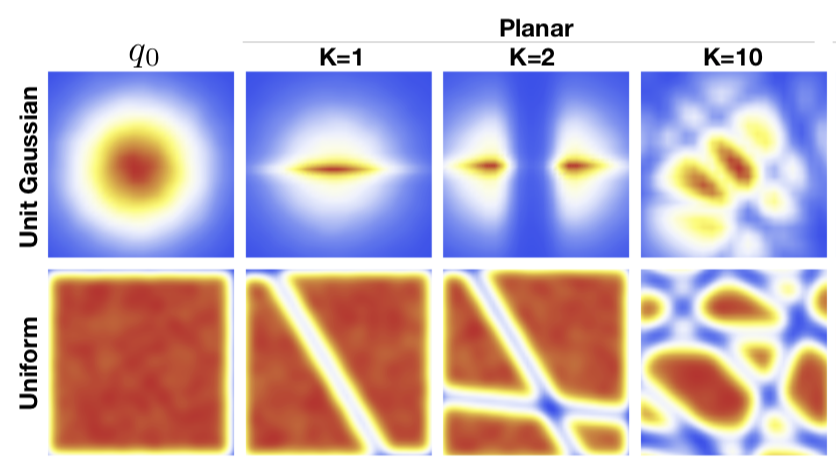
\includegraphics[width=0.8\linewidth]{figs/planar_flows.png}
	\end{figure}
	\end{block}
	\myfootnotewithlink{https://arxiv.org/abs/1505.05770}{Rezende D. J., Mohamed S. Variational Inference with Normalizing Flows, 2015} 
\end{frame}
%=======
\begin{frame}{Jacobian structure}

	\begin{block}{Flow likelihood}
		\[
		\log p(\bx|\btheta) = \log p(f(\bx, \btheta)) + \log \left|\det \left( \frac{\partial f(\bx, \btheta)}{\partial \bx} \right) \right|
		\]
	\end{block}
	\begin{itemize}
		\item What is a determinant of a diagonal matrix?
		\[
		\bz = f(\bx, \btheta) = (f_1(x_1, \btheta), \dots, f_m(x_m, \btheta)).
		\]
		\[
		\log \left|\det \left( \frac{\partial f(\bx, \btheta)}{\partial \bx} \right) \right| = \log \left| \prod_{i=1}^m f_i'(x_i, \btheta) \right| = \sum_{i=1}^m \log \left| f_i'(x_i, \btheta) \right|.
		\]
		\item What is a determinant of a triangular matrix? \\
		Let $z_i$ depends only on $\bx_{1:i}$ (or without loss of generality $x_i$ depends on $\bz_{1:i}$). \\
		What is the Jacobian of such a transformation?
	\end{itemize}
\end{frame}
%=======
\begin{frame}{NICE}
	\begin{block}{Coupling layer}
		\begin{equation*}
			\begin{cases} \bz_{1:d} = \bx_{1:d} \\ \bz_{d:m} = \tau (\bx_{d:m}, c(\bx_{1:d}))\end{cases} \quad 
			\begin{cases} \bx_{1:d} = \bz_{1:d} \\ \bx_{d:m} = \tau^{-1} (\bz_{d:m}, c(\bz_{1:d}))\end{cases}
		\end{equation*}
		\begin{itemize}
			\item $c: \mathbb{R}^d \rightarrow \mathbb{R}^{k}$ -- coupling function (do not need to be invertible);
			\item $\tau : \mathbb{R}^{m - d} \times c(\mathbb{R}^d) \rightarrow \mathbb{R}^{m - d}$ -- coupling law.
			\item 
			\[
			\det \left( \frac{\partial \bz}{\partial \bx} \right) = \det 
			\begin{pmatrix}
				\bI_d & 0_{d \times m - d} \\
				\frac{\partial \bz_{d:m}}{\partial \bx_{1:d}} & \frac{\partial \bz_{d:m}}{\partial \bx_{d:m}}
			\end{pmatrix} = 
			\det \left( \frac{\partial \bz_{d:m}}{\partial \bx_{d:m}} \right)
			\]
		\end{itemize}
	\end{block}
	\myfootnotewithlink{https://arxiv.org/abs/1410.8516}{Dinh L., Krueger D., Bengio Y. NICE: Non-linear Independent Components Estimation, 2014}
\end{frame}
%=======
\begin{frame}{NICE}
	\begin{block}{Coupling layer}
		\vspace{-0.8cm}
		\begin{equation*}
			\begin{cases} \bz_{1:d} = \bx_{1:d}; \\ \bz_{d:m} = \tau (\bx_{d:m}, c(\bx_{1:d}));\end{cases} 
			\quad \Rightarrow \quad 
			\begin{cases} \bx_{1:d} = \bz_{1:d}; \\ \bx_{d:m} = \tau^{-1} (\bz_{d:m}, c(\bz_{1:d})).\end{cases}
		\end{equation*}
		\vspace{-0.5cm}
	\end{block}
	\begin{block}{Coupling function $c(\cdot)$}
		Any complex function (without restrictions). For example, neural network.
	\end{block}
	\begin{block}{Coupling law $\tau(\cdot, \cdot)$}
		\begin{itemize}
			\item $\tau(x, c) = x + c$ -- \textit{additive};
			\item $\tau(x, c) = x \odot c, \, c \neq 0$ -- multiplicative;
			\item $\tau(x, c) = x \odot c_1 + c_2, \, c_1 \neq 0$ -- affine.
		\end{itemize}
	\end{block}
	To obtain more flexible class of dictributions, stack more coupling layers (with different ordering of components!). \\
	
	\myfootnotewithlink{https://arxiv.org/abs/1410.8516}{Dinh L., Krueger D., Bengio Y. NICE: Non-linear Independent Components Estimation, 2014}
\end{frame}
%=======
\begin{frame}{NICE}
	\begin{block}{Coupling layer}
		\vspace{-0.6cm}
		\begin{equation*}
			\begin{cases} \bz_{1:d} = \bx_{1:d}; \\ \bz_{d:m} = \tau (\bx_{d:m}, c(\bx_{1:d}));\end{cases} 
			\quad \Rightarrow \quad 
			\begin{cases} \bx_{1:d} = \bz_{1:d}; \\ \bx_{d:m} = \tau^{-1} (\bz_{d:m}, c(\bz_{1:d})).\end{cases}
		\end{equation*}
		\vspace{-0.5cm}
	\end{block}
	\begin{block}{Jacobian}
			\vspace{-0.3cm}
		\[
		\det \left( \frac{\partial \bz}{\partial \bx} \right) = \det 
		\begin{pmatrix}
			\bI_d & 0_{d \times m - d} \\
			\frac{\partial \bz_{d:m}}{\partial \bx_{1:d}} & \frac{\partial \bz_{d:m}}{\partial \bx_{d:m}}
		\end{pmatrix} = 
		\det \left( \frac{\partial \bz_{d:m}}{\partial \bx_{d:m}} \right)
		\]
	\end{block}
	What is the Jacobian for the additive coupling law $\tau(x + c) = x + c$? \\
	In this case the transformation is \textit{volume preserving}. \\
	The last layer is rescaling $z_i = s_i x_i$ ($x_i = z_i / s_i$). \\
	What is the Jacobian of the last layer?
	\myfootnotewithlink{https://arxiv.org/abs/1410.8516}{Dinh L., Krueger D., Bengio Y. NICE: Non-linear Independent Components Estimation, 2014}
\end{frame}
%=======
\begin{frame}{NICE}
	\begin{figure}
		\centering
		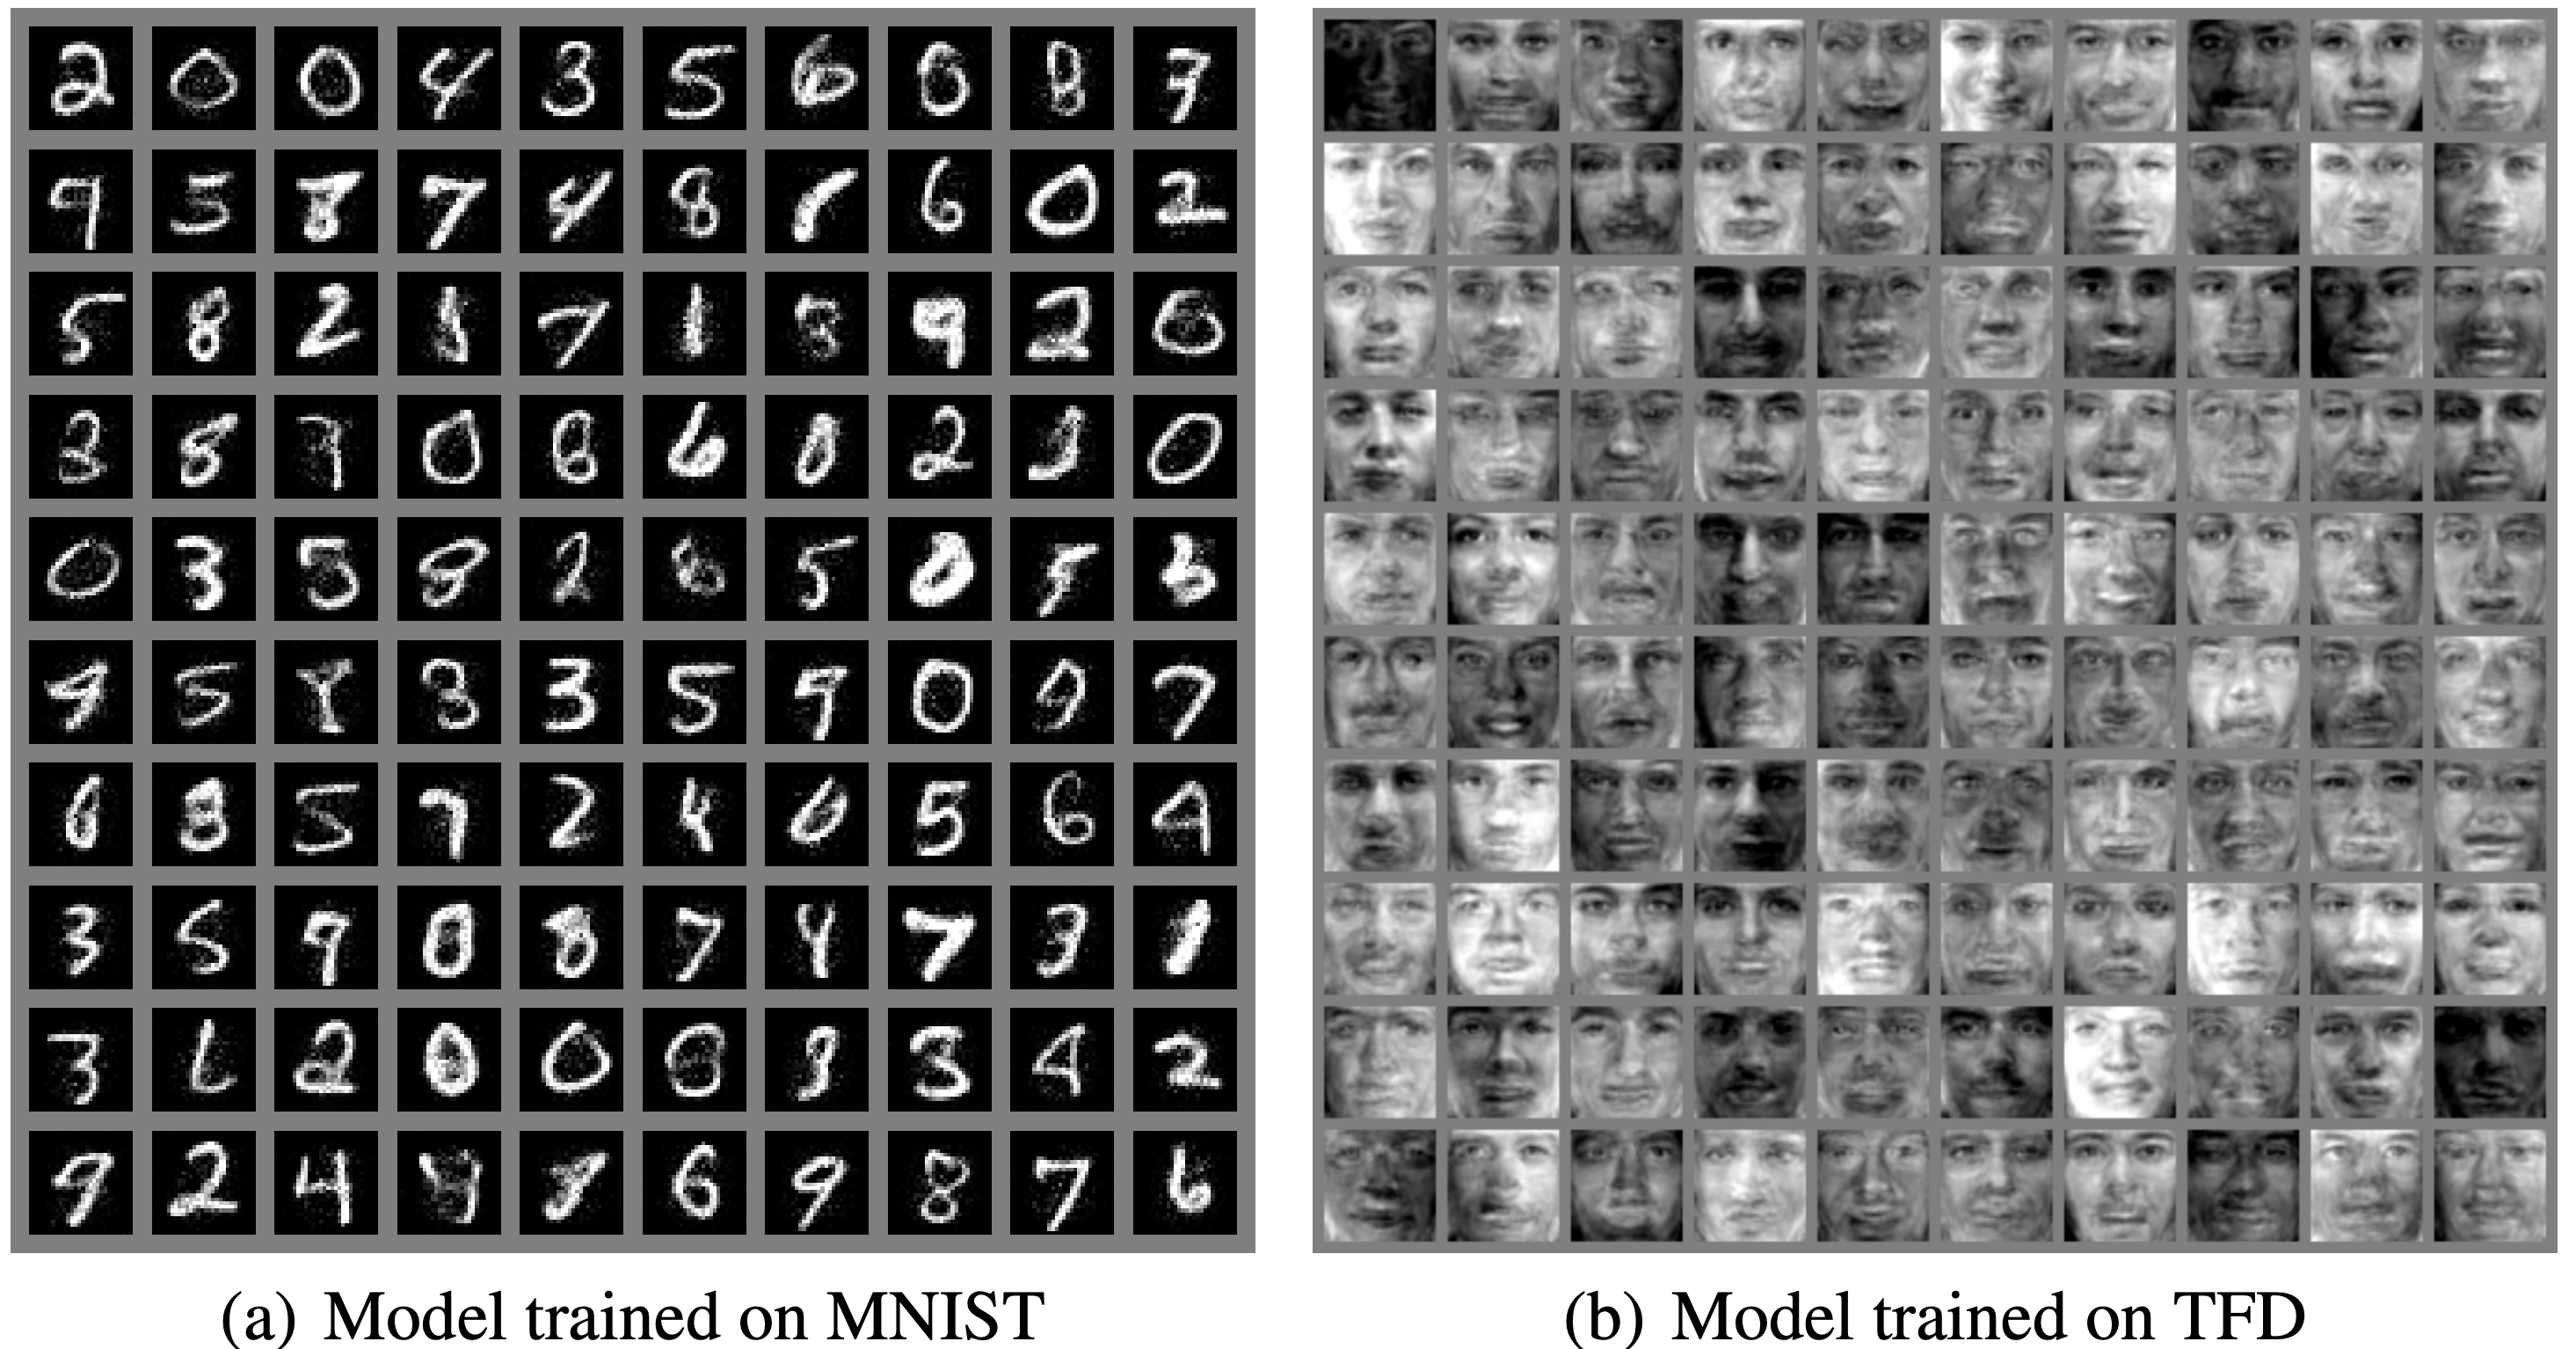
\includegraphics[width=\linewidth]{figs/nice_results.png}
	\end{figure}
	\myfootnotewithlink{https://arxiv.org/abs/1410.8516}{Dinh L., Krueger D., Bengio Y. NICE: Non-linear Independent Components Estimation, 2014}
\end{frame}
%=======
\begin{frame}{RealNVP}
	\begin{block}{Affine coupling law}
		\[
		\begin{cases} \bz_{1:d} = \bx_{1:d}; \\ \bz_{d:m} = \bx_{d:m} \odot \exp \left(c_1(\bx_{1:d}, \btheta)\right) + c_2(\bx_{1:d}, \btheta).\end{cases} 
		\]
		\[
		\begin{cases} \bx_{1:d} = \bz_{1:d}; \\ \bx_{d:m} = \left(\bz_{d:m} - c_2(\bx_{1:d}, \btheta) \right) \odot \exp(-c_1(\bx_{1:d}, \btheta)).\end{cases}
		\]
	\end{block}
	\begin{block}{Jacobian}
		\vspace{-0.3cm}
		\[
		\det \left( \frac{\partial \bz}{\partial \bx} \right) = \det 
		\begin{pmatrix}
			\bI_d & 0_{d \times m - d} \\
			\frac{\partial \bz_{d:m}}{\partial \bx_{1:d}} & \frac{\partial \bz_{d:m}}{\partial \bx_{d:m}}
		\end{pmatrix} = \prod_{i=1}^{m - d} \exp (c_1(\bx_{1:d}, \btheta)_i).
		\]
		Non-Volume Preserving.
	\end{block}
	
		\myfootnotewithlink{https://arxiv.org/abs/1605.08803}{Dinh L., Sohl-Dickstein J., Bengio S. Density estimation using Real NVP, 2016} 
\end{frame}
%=======
\begin{frame}{RealNVP}
	\begin{block}{Affine coupling law}
		\[
		\begin{cases} \bz_{1:d} = \bx_{1:d}; \\ \bz_{d:m} = \bx_{d:m} \odot \exp \left(c_1(\bx_{1:d}, \btheta)\right) + c_2(\bx_{1:d}, \btheta).\end{cases} 
		\]
	\end{block}
	How to choose variable partitioning for images?
	\begin{figure}
		\centering
		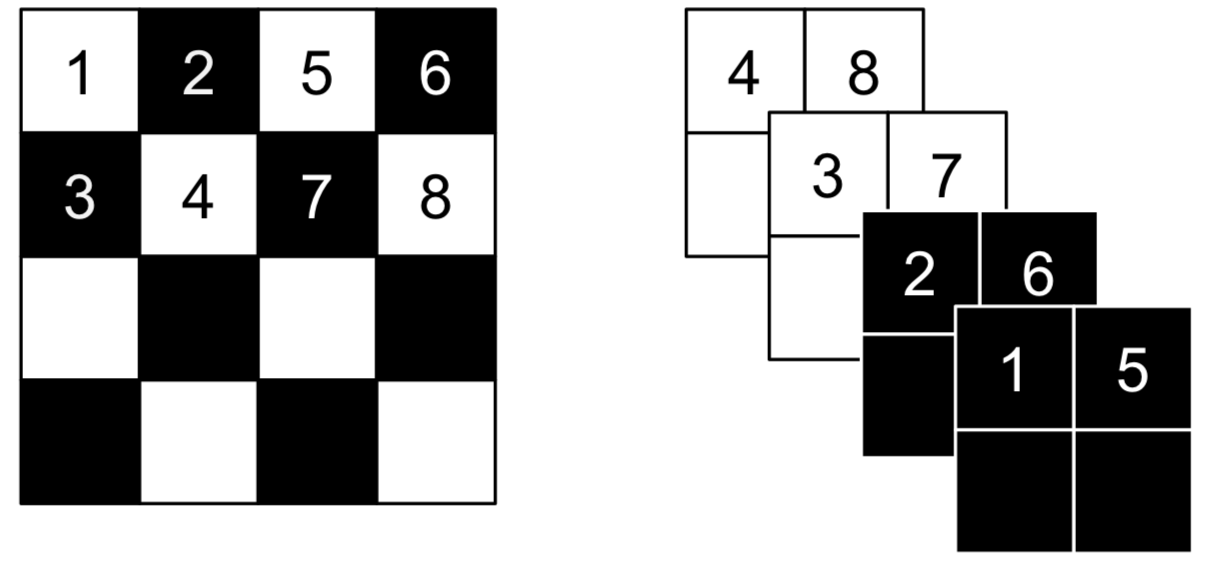
\includegraphics[width=0.75\linewidth]{figs/realnvp_masking.png}
	\end{figure}
	Masked convolutions are used to define ordering.
	
	\myfootnotewithlink{https://arxiv.org/abs/1605.08803}{Dinh L., Sohl-Dickstein J., Bengio S. Density estimation using Real NVP, 2016} 
\end{frame}
%=======
\begin{frame}{RealNVP}
	\begin{figure}
		\centering
		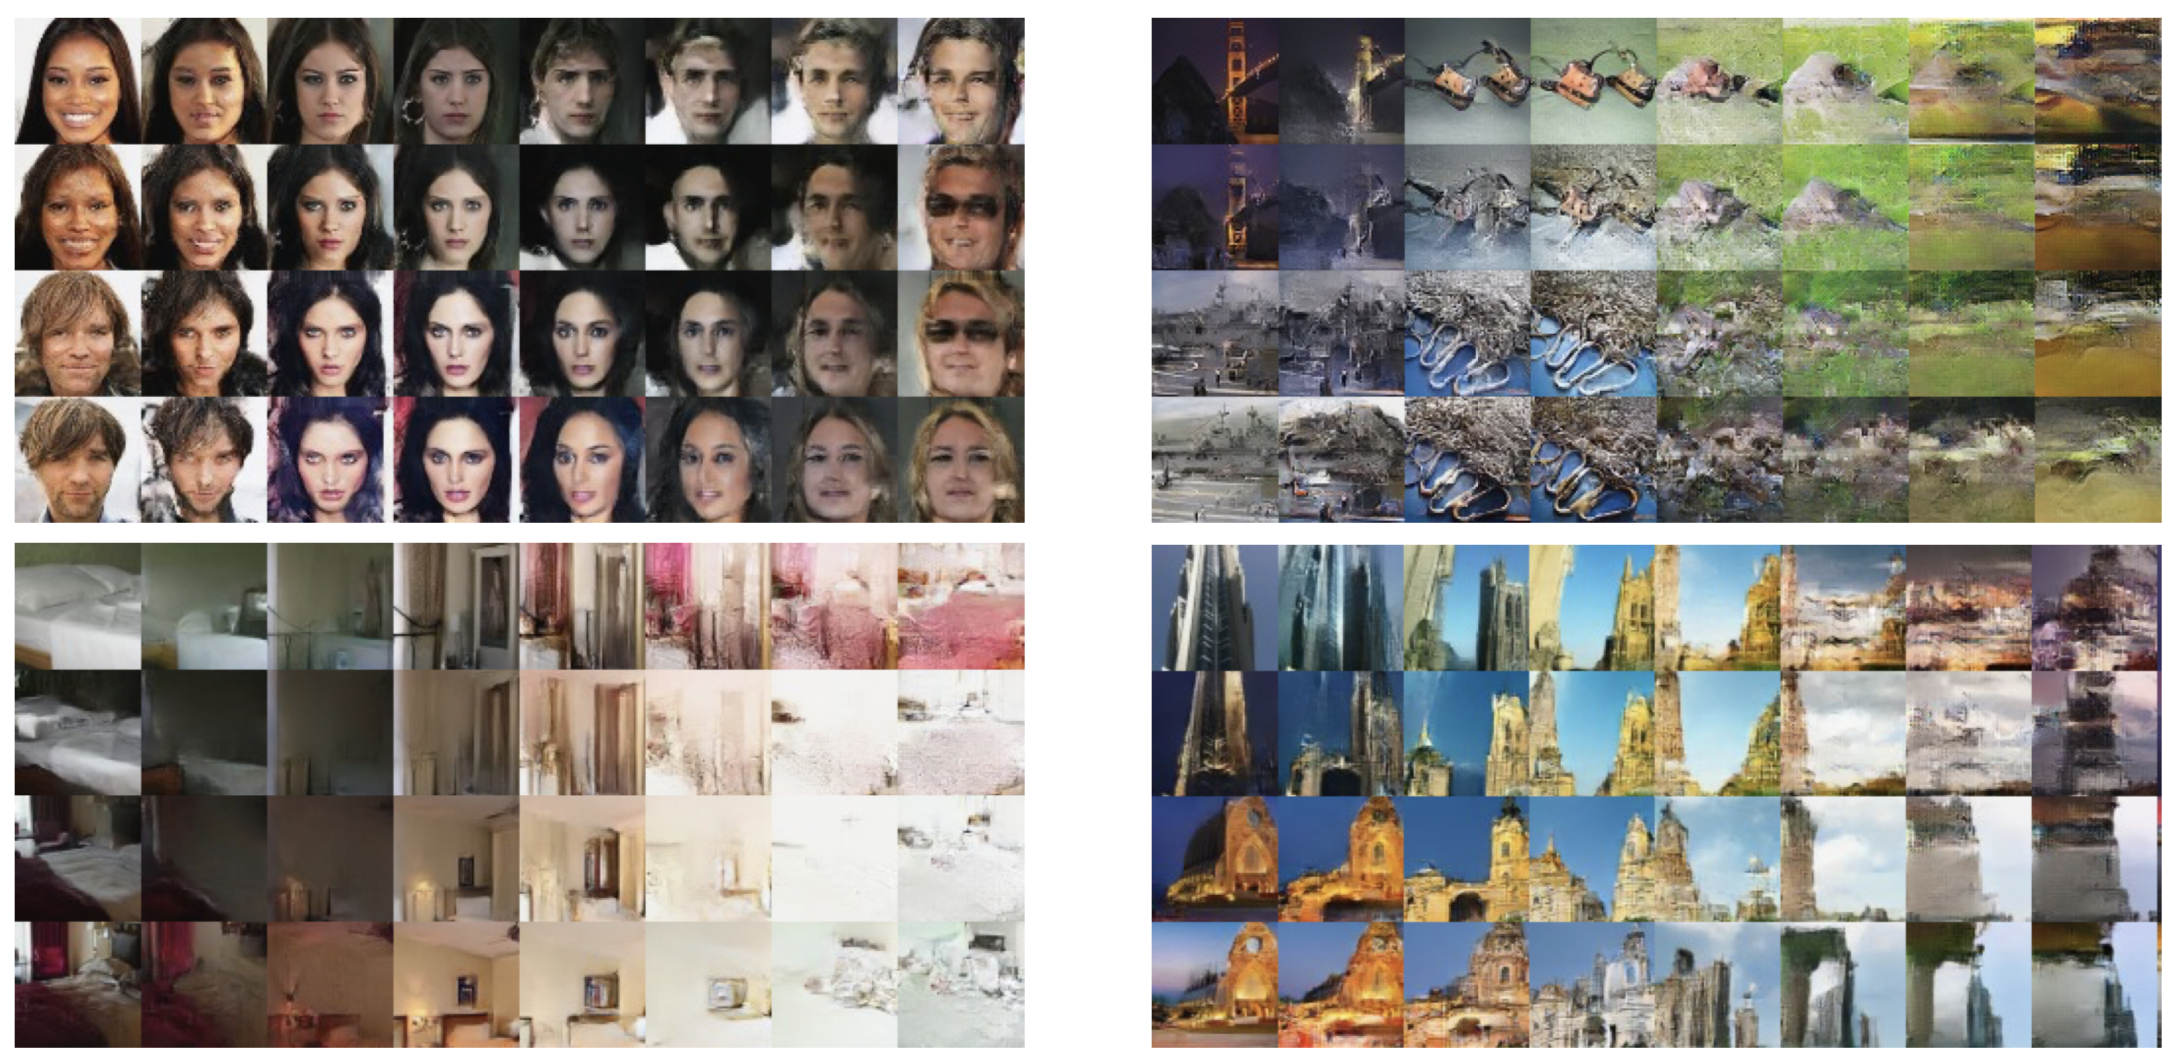
\includegraphics[width=\linewidth]{figs/realnvp_output.png}
	\end{figure}
	\myfootnotewithlink{https://arxiv.org/abs/1605.08803}{Dinh L., Sohl-Dickstein J., Bengio S. Density estimation using Real NVP, 2016} 
\end{frame}
%=======
\begin{frame}{RevNets, 2017}
	\begin{minipage}[t]{0.6\columnwidth}
		\begin{itemize}
			\item Modern neural networks are trained via backpropagation.
			\item Residual networks are state of the art in image classification.
			\item Backpropagation requires storing the network activations.
		\end{itemize}
	\end{minipage}%
	\begin{minipage}[t]{0.4\columnwidth}
		\begin{figure}
			\centering
			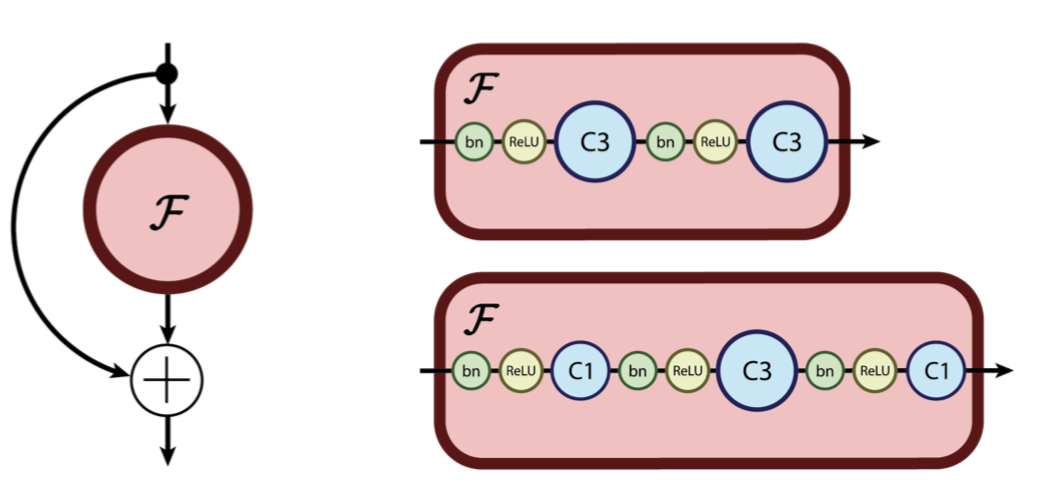
\includegraphics[width=\linewidth]{figs/resnet_block.png}
		\end{figure}
	\end{minipage}
	\vspace{0.1cm}
	\begin{block}{Problem}
		Storing the activations imposes an increasing memory burden. GPUs have limited memory capacity, leading to constraints often exceeded by state-of-the-art architectures (with thousand layers).
	\end{block}
	\myfootnotewithlink{https://arxiv.org/abs/1707.04585}{Gomez A. N. et al. The Reversible Residual Network: Backpropagation Without Storing Activations, 2017}
\end{frame}
%=======
\begin{frame}{RevNets, 2017}
	\begin{block}{NICE}
		\vspace{-0.2cm}
		\begin{equation*}
			\begin{cases} \bz_1 = \bx_1; \\ \bz_2 = \bx_2 + \mathcal{F}(\bx_1, \btheta);\end{cases}  \quad \Leftrightarrow \quad 
			\begin{cases} \bx_1 = \bz_1; \\ \bx_2 = \bz_2 - \mathcal{F}(\bz_1, \btheta).\end{cases} 
		\end{equation*}
		\vspace{-0.2cm}
	\end{block}
	\begin{block}{RevNet}
		\begin{equation*}
			\begin{cases} \by_1 = \bx_1 + \mathcal{F}(\bx_2, \btheta); \\ \by_2 = \bx_2 + \mathcal{G}(\by_1, \btheta);\end{cases} \quad \Leftrightarrow \quad 
			\begin{cases} \bx_2 = \by_2 - \mathcal{F}(\by_1, \btheta); \\ \bx_1 = \by_1 - \mathcal{G}(\bx_2, \btheta).\end{cases} 
		\end{equation*}
	\end{block}
	\begin{figure}
		\centering
		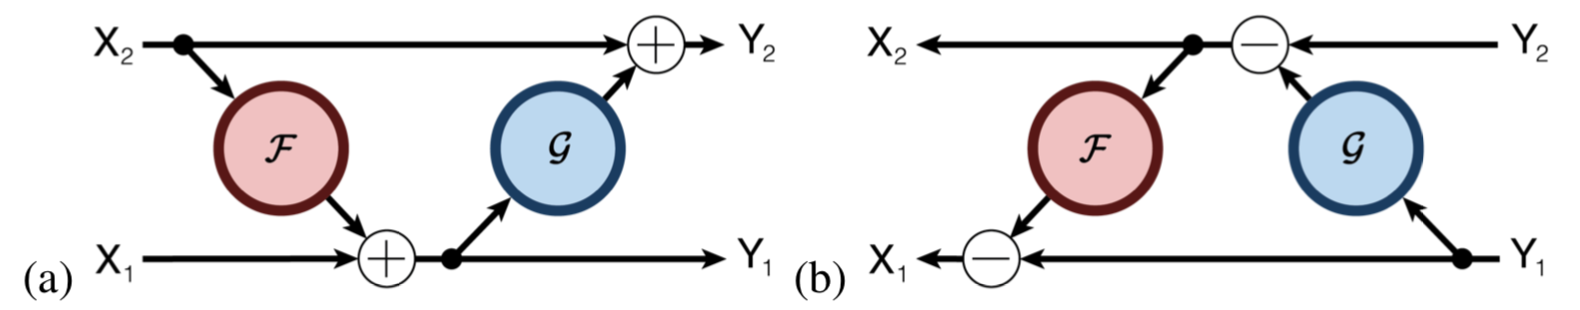
\includegraphics[width=\linewidth]{figs/revnet.png}
	\end{figure}
	\myfootnotewithlink{https://arxiv.org/abs/1707.04585}{Gomez A. N. et al. The Reversible Residual Network: Backpropagation Without Storing Activations, 2017}
\end{frame}
%=======
\begin{frame}{RevNets, 2017}
	\begin{figure}
		\centering
		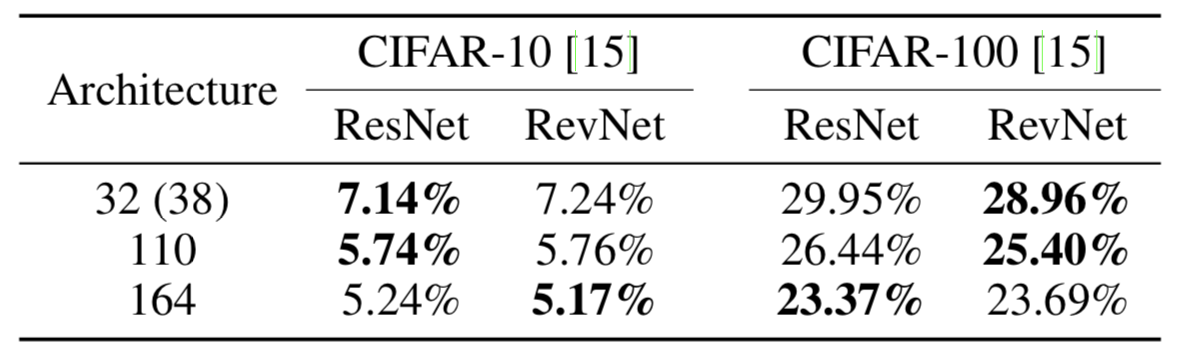
\includegraphics[width=0.8\linewidth]{figs/revnet_results.png}
	\end{figure}
	\begin{itemize}
		\item If the network contains non-reversible blocks (poolings, strides), activations for these blocks should be stored.
		\item To avoid storing activations in the modern frameworks, the backward pass should be manually redefined.
	\end{itemize}
	\myfootnotewithlink{https://arxiv.org/abs/1707.04585}{Gomez A. N. et al. The Reversible Residual Network: Backpropagation Without Storing Activations, 2017}
\end{frame}
%=======
\begin{frame}{i-RevNet, 2018}
	\begin{block}{Hypothesis}
		The success of deep convolutional networks is based on progressively discarding uninformative variability about the input with respect to the problem at hand. 
	\end{block}
	\begin{itemize}
		\item It is difficult to recover images from their hidden representations. 
		\item Information bottleneck principle: an optimal representation must reduce the MI between an input and its representation to reduce uninformative variability + maximize the MI between the output and its representation to preserve each class from collapsing onto other classes.
	\end{itemize}
	\myfootnotewithlink{https://arxiv.org/abs/1802.07088}{Jacobsen J. H., Smeulders A., Oyallon E. i-RevNet: Deep Invertible Networks, 2018}
\end{frame}
%=======
\begin{frame}{i-RevNet, 2018}
	\begin{block}{Hypothesis}
		The success of deep convolutional networks is based on progressively discarding uninformative variability about the input with respect to the problem at hand. 
	\end{block}
	
	\begin{block}{Idea}
		Build a cascade of homeomorphic layers (i-RevNet), a network that can be fully inverted up to the final projection onto the classes, i.e. no information is discarded.
	\end{block}
	\myfootnotewithlink{https://arxiv.org/abs/1802.07088}{Jacobsen J. H., Smeulders A., Oyallon E. i-RevNet: Deep Invertible Networks, 2018}
\end{frame}
%=======
\begin{frame}{i-RevNet, 2018}
	
	\begin{figure}
		\centering
		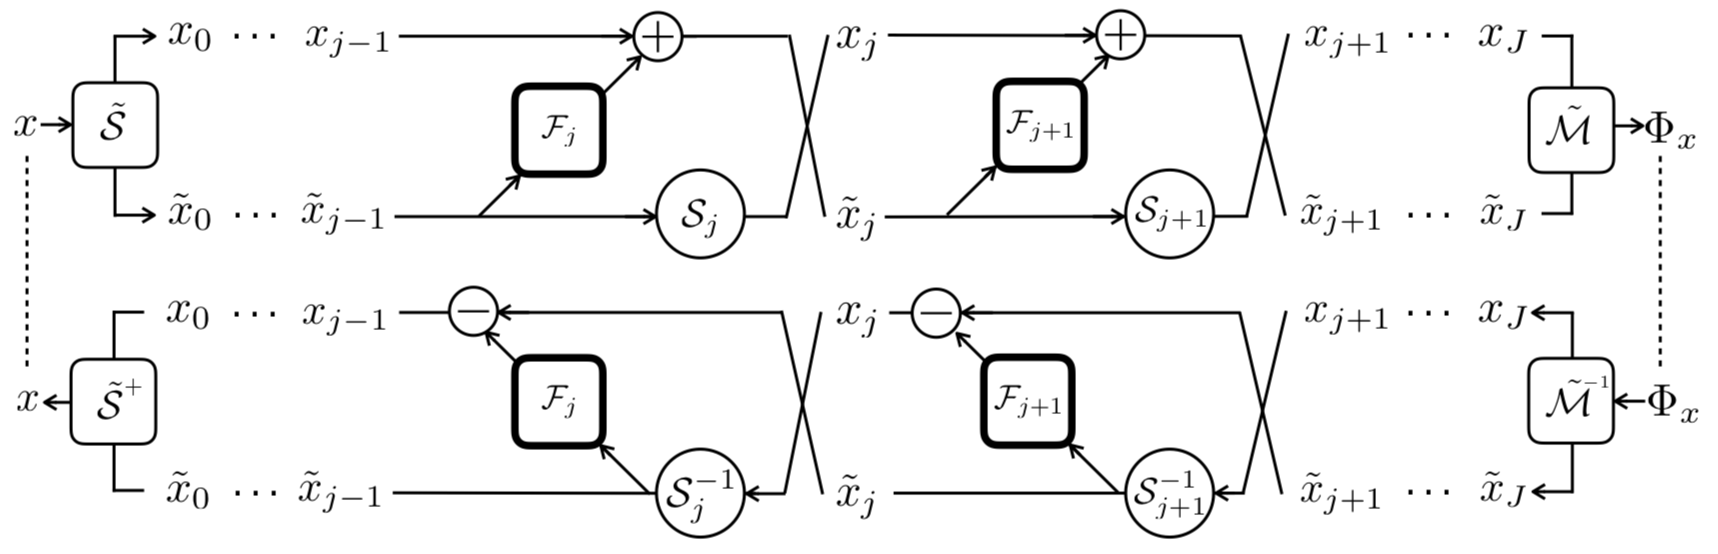
\includegraphics[width=\linewidth]{figs/i-revnet.png}
	\end{figure}
	
	\begin{figure}
		\centering
		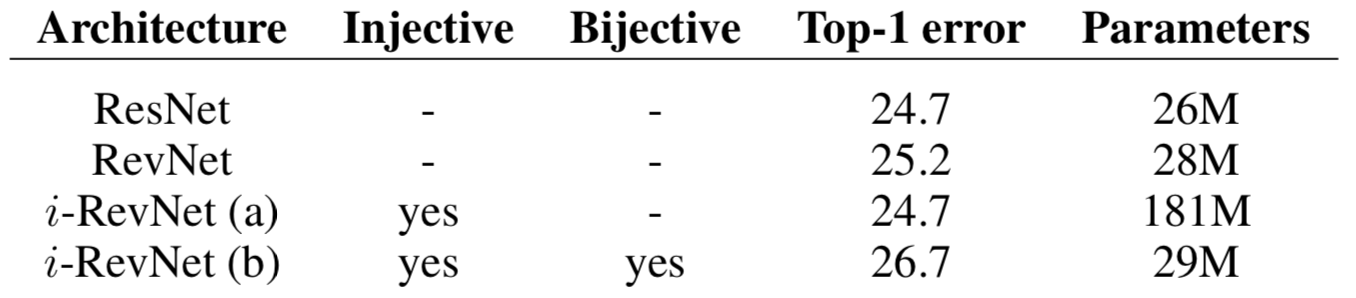
\includegraphics[width=0.9\linewidth]{figs/i-revnet_block.png}
	\end{figure}

	\myfootnotewithlink{https://arxiv.org/abs/1802.07088}{Jacobsen J. H., Smeulders A., Oyallon E. i-RevNet: Deep Invertible Networks, 2018}
\end{frame}
%=======
\begin{frame}{Glow, 2018}
	\begin{figure}
		\centering
		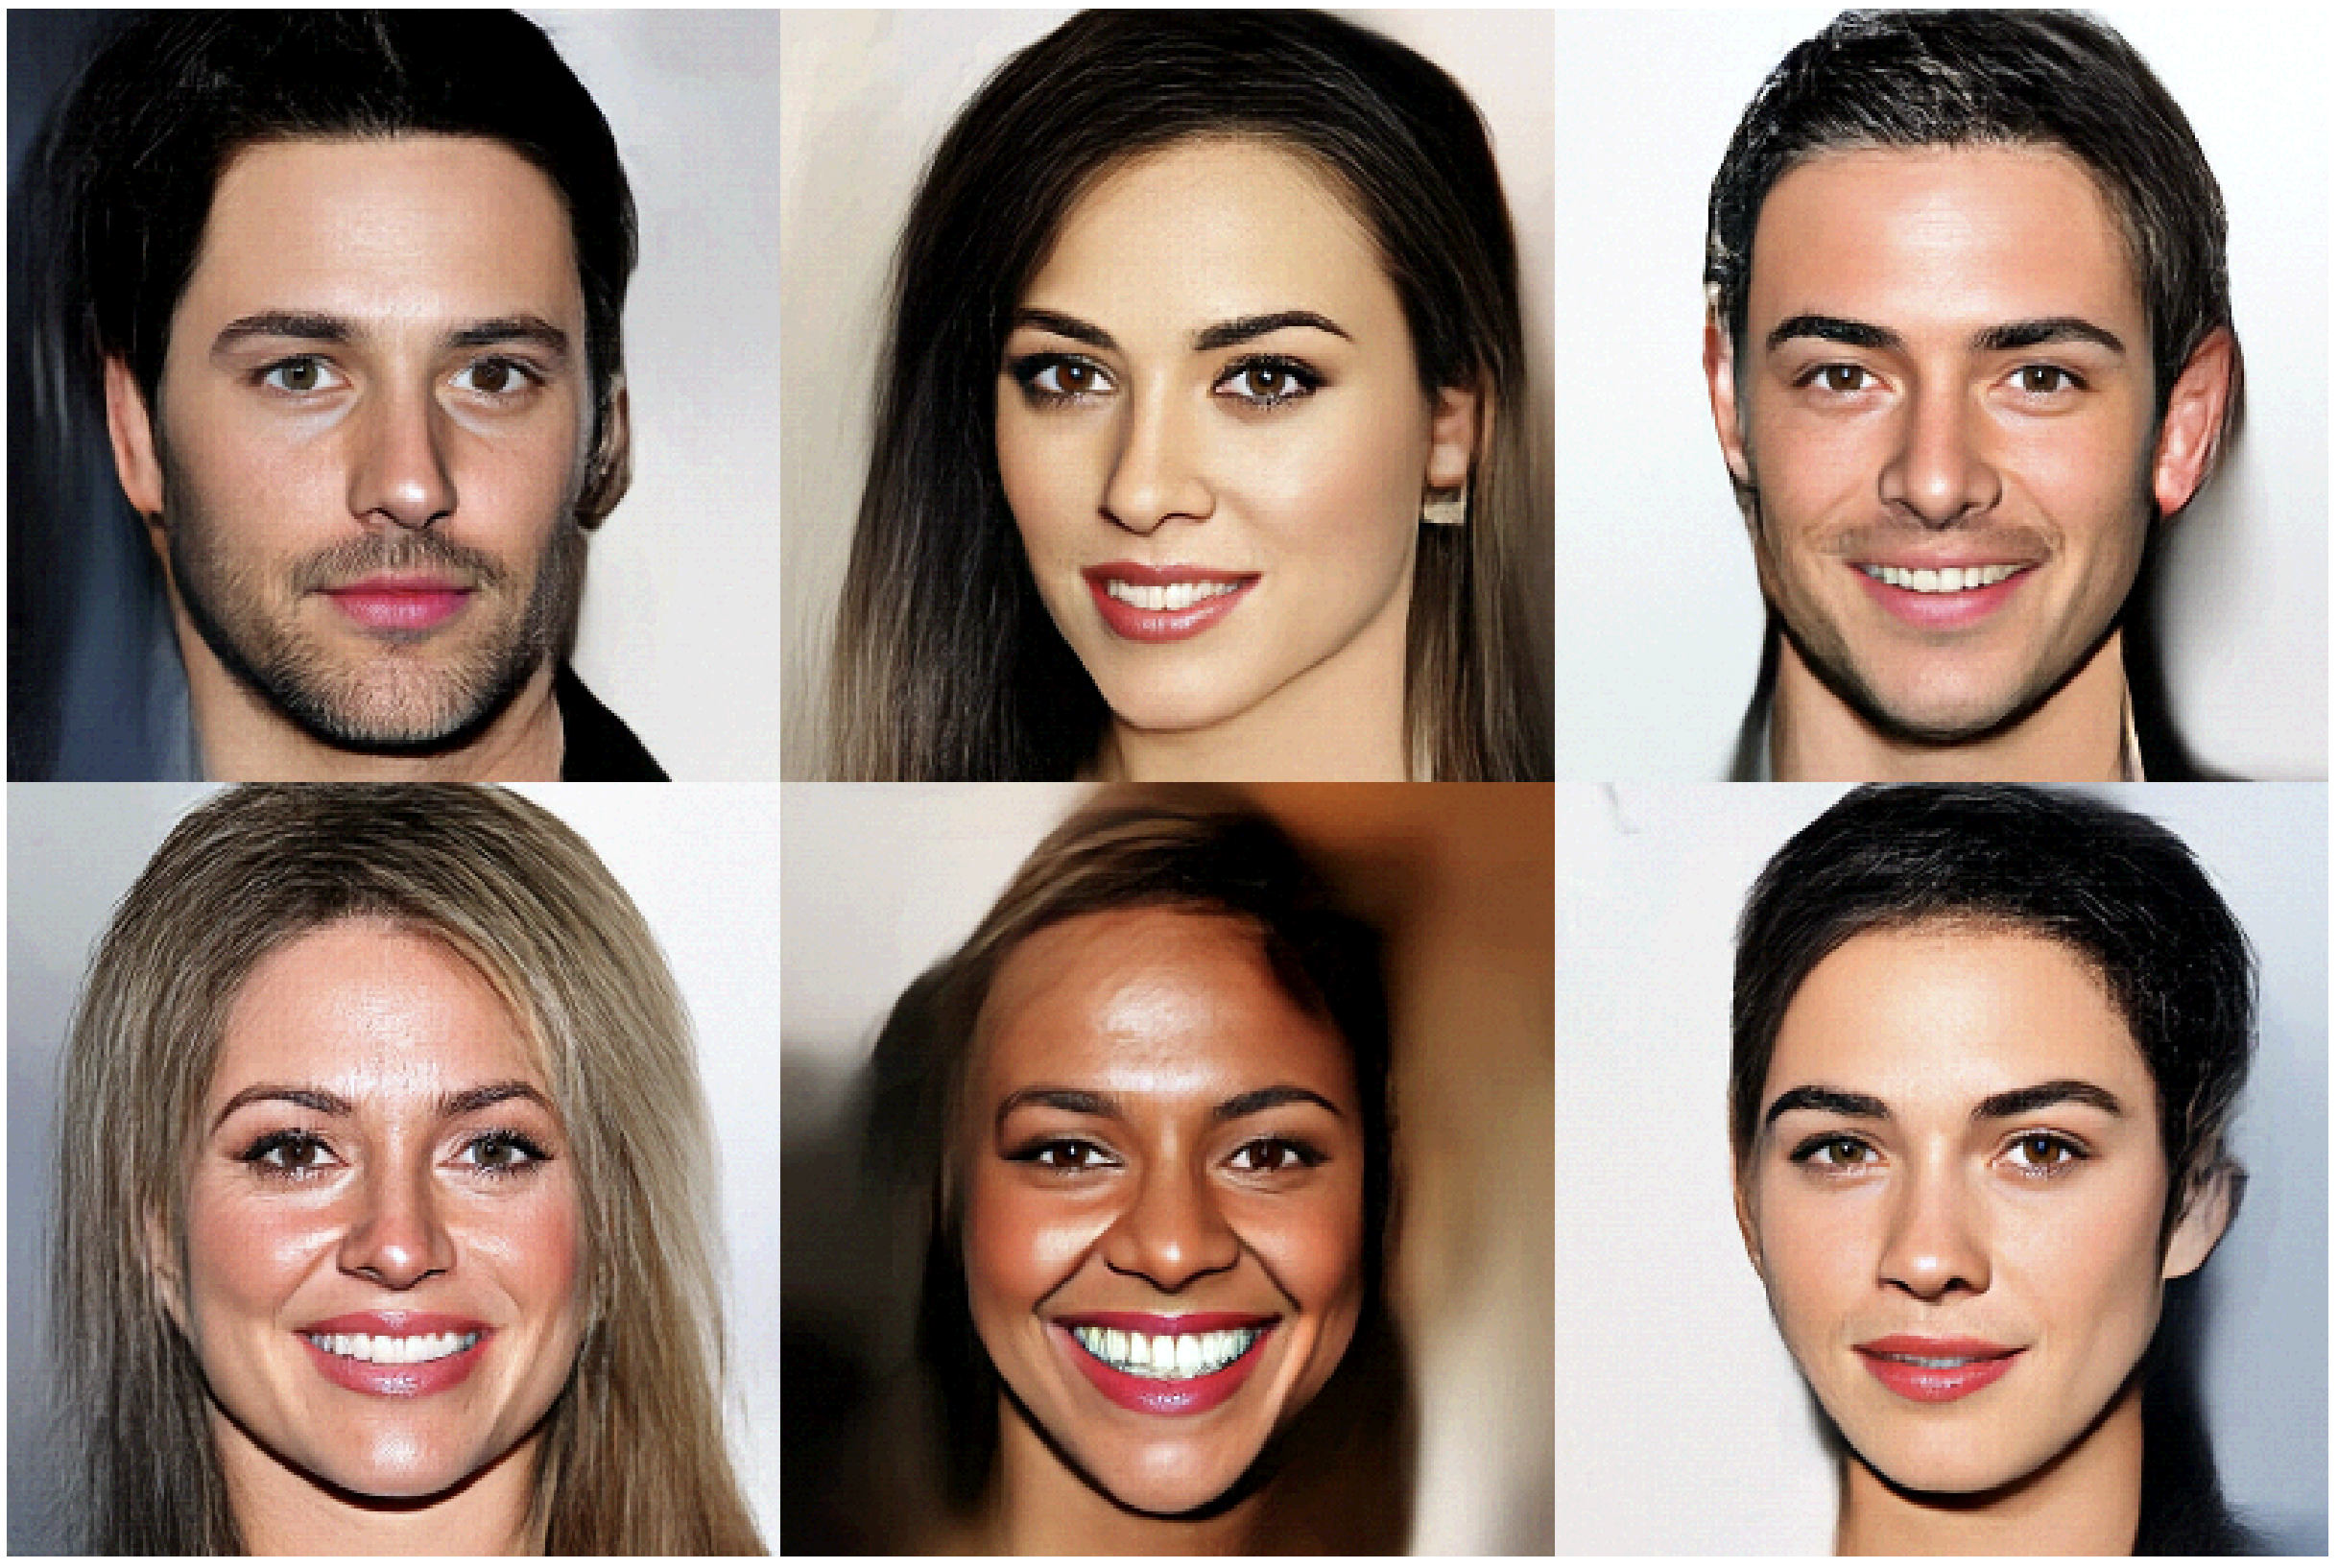
\includegraphics[width=\linewidth]{figs/glow_faces.png}
	\end{figure}
	\myfootnotewithlink{https://arxiv.org/abs/1807.03039}{Kingma D. P., Dhariwal P. Glow: Generative Flow with Invertible 1x1 Convolutions, 2018}
\end{frame}
%=======
\begin{frame}{Glow, 2018}
	\begin{block}{Model architecture}
		\begin{figure}
			\centering
			\includegraphics[width=\linewidth]{figs/glow_block.png}
		\end{figure}
	\end{block}
	\myfootnotewithlink{https://arxiv.org/abs/1807.03039}{Kingma D. P., Dhariwal P. Glow: Generative Flow with Invertible 1x1 Convolutions, 2018}
\end{frame}
%=======
\begin{frame}{Glow, 2018}
	
	\begin{block}{NICE}
		\vspace{-0.2cm}
		\begin{equation*}
			\begin{cases} \bz_1 = \bx_1; \\ \bz_2 = \bx_2 + \mathcal{F}(\bx_1, \btheta);\end{cases}  \quad \Leftrightarrow \quad 
			\begin{cases} \bx_1 = \bz_1; \\ \bx_2 = \bz_2 - \mathcal{F}(\bz_1, \btheta).\end{cases} 
		\end{equation*}
		\vspace{-0.2cm}
	\end{block}
	
	First step is \textbf{split} operator which decouples a variable into 2 subparts (usualy channel-wise).
	The order of decoupling should be manually changed between layers.
	
	Could we use more general operator?
	
	Let use rotation matrix via 1x1 invertible convolution.
	
	$\mathbf{W} \in \mathbb{R}^{c \times c}$ - kernel of 1x1 convolution with $c$ input and output channels.
	
	The cost of computing or differentiating $\det (\mathbf{W})$ is $O(c^3)$.

	\myfootnotewithlink{https://arxiv.org/abs/1807.03039}{Kingma D. P., Dhariwal P. Glow: Generative Flow with Invertible 1x1 Convolutions, 2018}
\end{frame}
%=======
\begin{frame}{Glow, 2018}
	\begin{figure}
		\centering
		\includegraphics[width=\linewidth]{figs/glow_ops.png}
	\end{figure}

	\myfootnotewithlink{https://arxiv.org/abs/1807.03039}{Kingma D. P., Dhariwal P. Glow: Generative Flow with Invertible 1x1 Convolutions, 2018}
\end{frame}
%=======
\begin{frame}{Glow, 2018}
	\begin{block}{Invertible 1x1 conv}
		Cost to compute $\det (\mathbf{W})$ is $O(c^3)$. 
		LU-decomposition reduces the cost to $O(c)$:
		\[
		\mathbf{W} = \mathbf{P}\mathbf{L}(\mathbf{U} + \text{diag}(\mathbf{s})),
		\]
		where $\mathbf{P}$ is a permutation matrix, $\mathbf{L}$ is a lower triangular matrix with ones on the diagonal, $\mathbf{U}$ is an
		upper triangular matrix with zeros on the diagonal, and $\mathbf{s}$ is a vector.
	\end{block}
	\begin{figure}
		\centering
		\includegraphics[width=\linewidth]{figs/glow_1x1_conv.png}
	\end{figure}

	\myfootnotewithlink{https://arxiv.org/abs/1807.03039}{Kingma D. P., Dhariwal P. Glow: Generative Flow with Invertible 1x1 Convolutions, 2018}  
\end{frame}
%=======
\begin{frame}{Glow, 2018}
	\begin{block}{Face interpolation}
		\begin{figure}
			\centering
			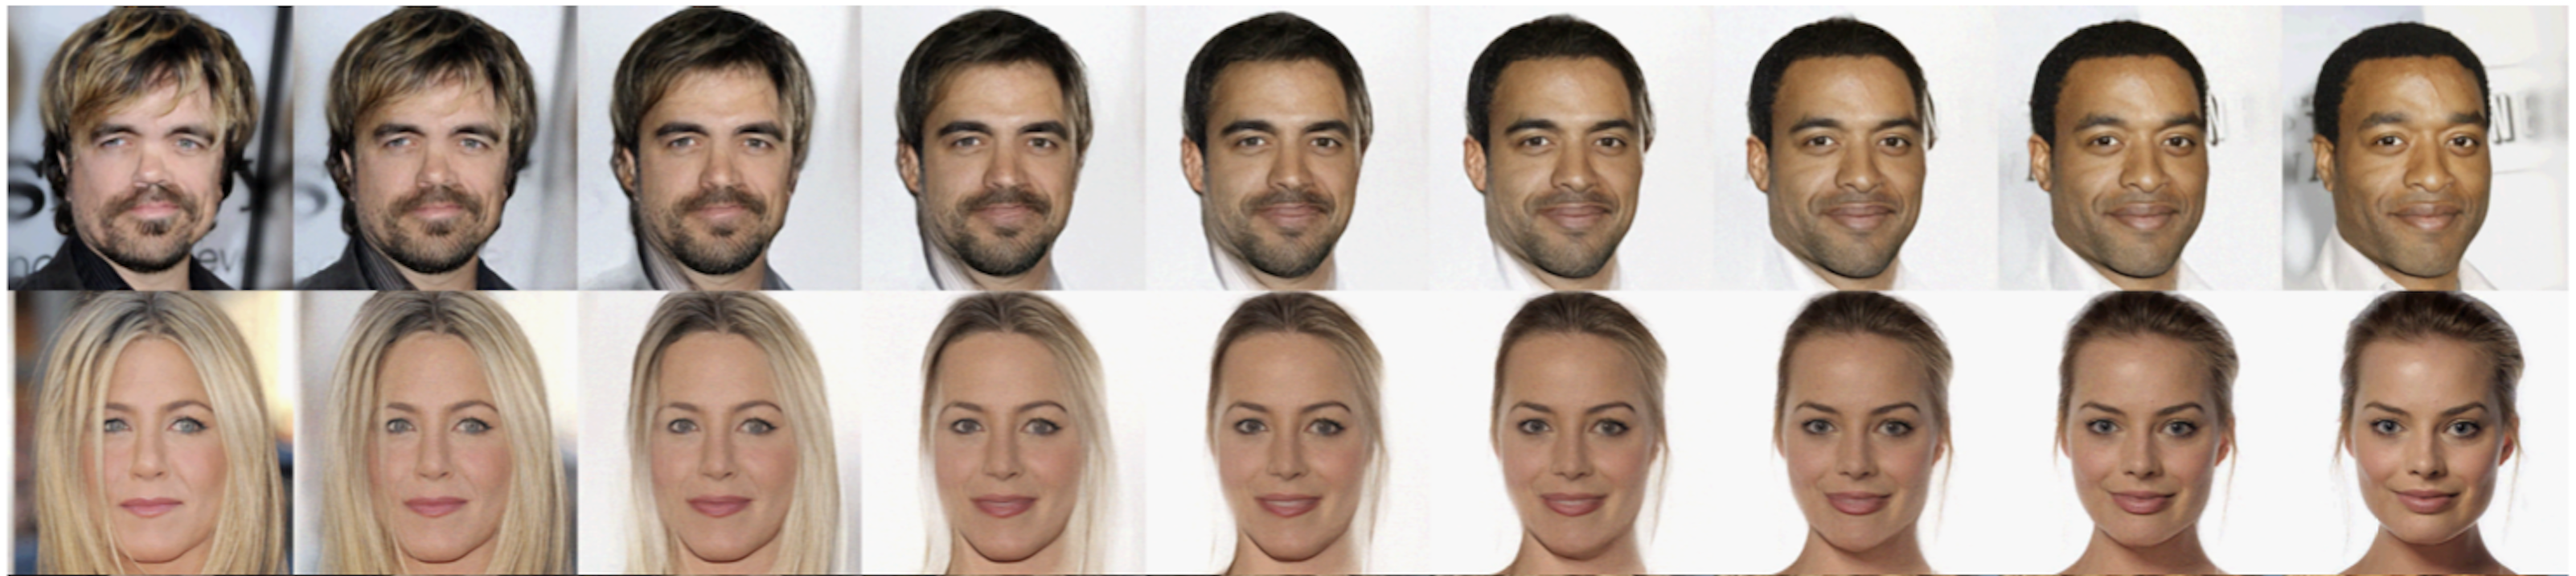
\includegraphics[width=\linewidth]{figs/glow_interpolation.png}
		\end{figure}
	\end{block}

	\myfootnotewithlink{https://arxiv.org/abs/1807.03039}{Kingma D. P., Dhariwal P. Glow: Generative Flow with Invertible 1x1 Convolutions, 2018}
\end{frame}
%=======
\begin{frame}{Glow, 2018}
	\begin{block}{Face attributes manipulation}
		\begin{figure}
			\centering
			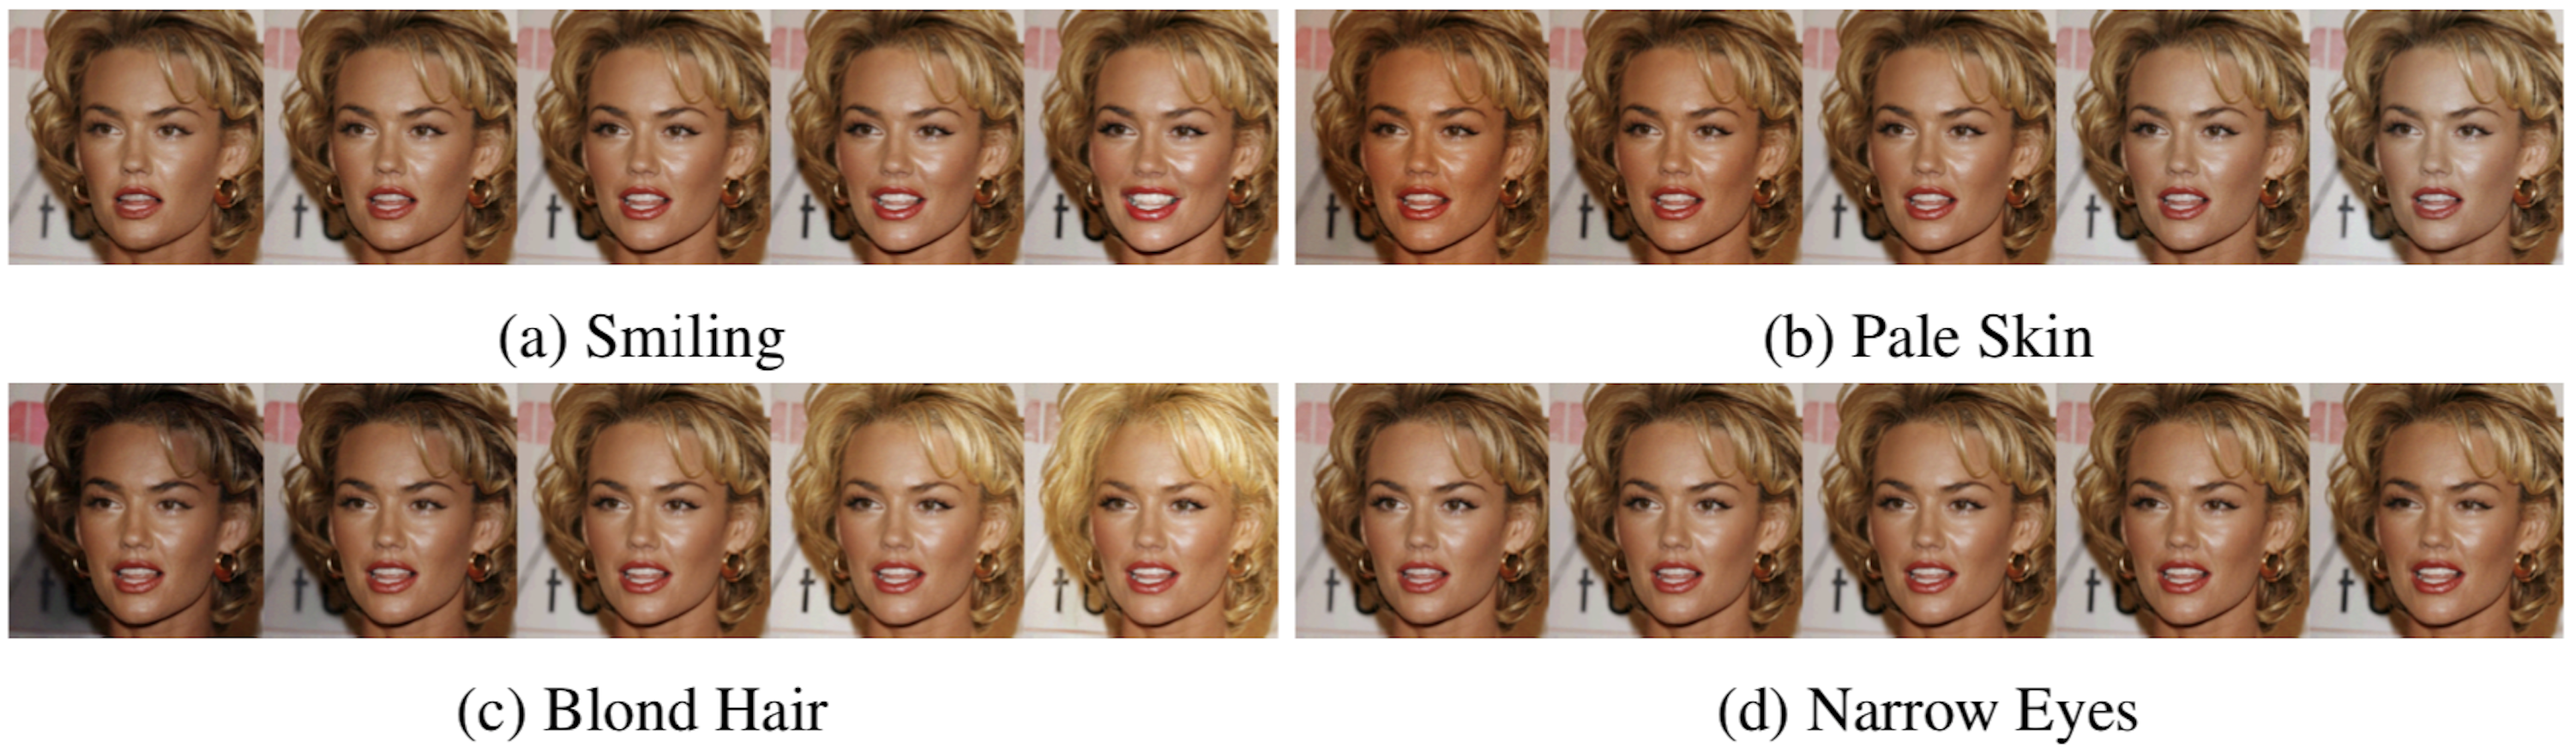
\includegraphics[width=\linewidth]{figs/glow_attributes.png}
		\end{figure}
	\end{block}

	\myfootnotewithlink{https://arxiv.org/abs/1807.03039}{Kingma D. P., Dhariwal P. Glow: Generative Flow with Invertible 1x1 Convolutions, 2018} 
\end{frame}
\begin{frame}{Summary}
	\begin{itemize}
		\item Flows are generative models with tractable likelihood and latent representation.
		\item Flows transform simple distributions into the complex ones via sequences of invertible transformations.
		\item The goal is to achieve tractable Jacobian for efficient learning and density estimation.
	\end{itemize}
\end{frame}
%=======
\begin{frame}{Dequantization}
	\begin{itemize}
		\item Images are discrete data (pixels lies in the [0, 255] integer domain). 
		\item Flow is a continuous model.
	\end{itemize}
	Fitting a continuous density model to discrete data, produces a degenerate solution with all probability mass on discrete values. \\
	How to convert discrete data distribution to the continuous one?
	
	\begin{minipage}[t]{0.5\columnwidth}
		\begin{block}{Uniform dequantization}
			\[
			\by = \bx + \bu, \quad \bu \sim U[0, 1]
			\]
		\end{block}
	\end{minipage}%
	\begin{minipage}[t]{0.5\columnwidth}
		\begin{figure}
			\centering
			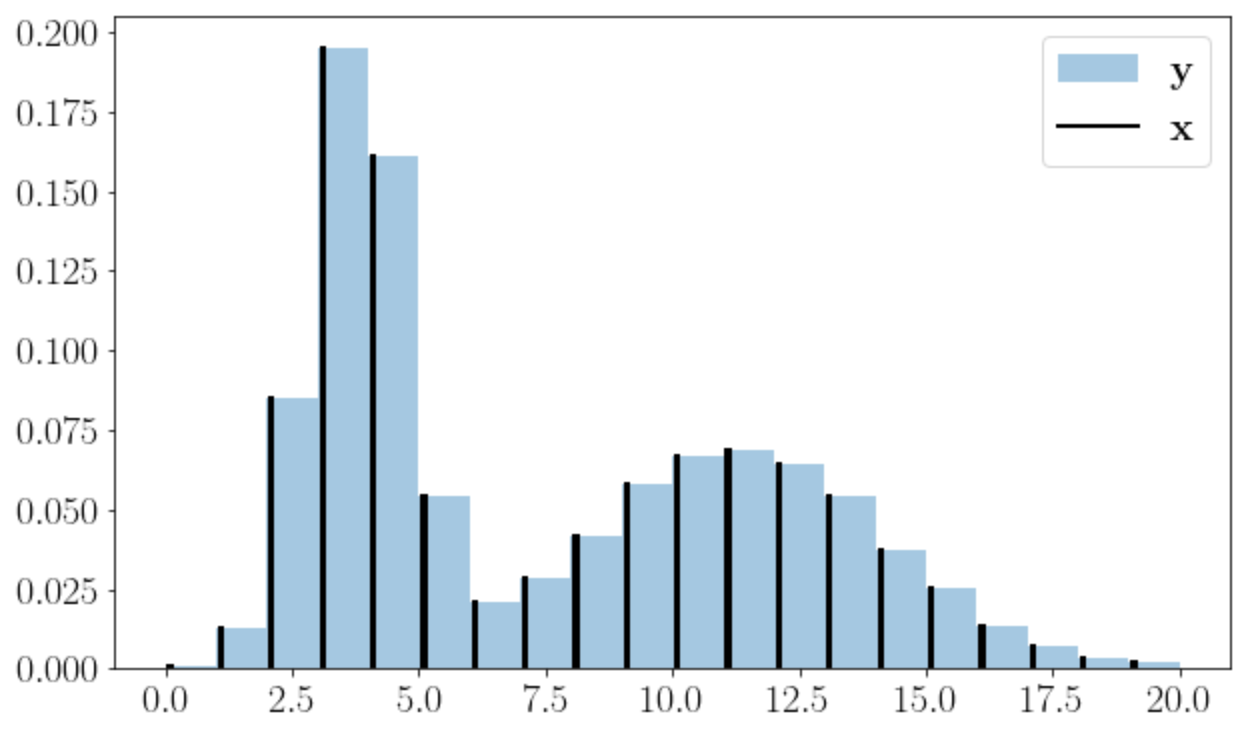
\includegraphics[width=1.0\linewidth]{figs/uniform_dequantization.png}
		\end{figure}
	\end{minipage}
\end{frame}
%=======
\begin{frame}{Uniform dequantization}
	\begin{block}{Statement}
		Fitting continious model $p(\by | \btheta)$ on uniformly dequantized data $\by = \bx + \bu, \, \bu \sim U[0, 1]$ is equivalent to maximization of a lower bound on the log-likelihood for a discrete model:
		\[
		P(\bx | \btheta) = \int_{U[0, 1]} p(\bx + \bu | \btheta) d \bu
		\]
		\vspace{-0.2cm} \\
		Thus, maximizing the log-likelihood of the continuous model on $\by$ cannot lead to the collapsing onto the discrete data (objective is bounded above by the log-likelihood of a discrete model).
	\end{block}
	\begin{block}{Proof}
		\vspace{-1cm}
		\begin{multline*}
			\log p(\bY | \btheta) = \sum_{i = 1}^n \log p(\by_i | \btheta) = \sum_{i = 1}^n \int_{U[0, 1]} \log p(\bx_i + \bu | \btheta) d \bu \\ \leq \sum_{i = 1}^n \log \int_{U[0, 1]} p(\bx_i + \bu | \btheta) d \bu = \sum_{i=1}^n \log P(\bx_i | \btheta).
		\end{multline*}
	\end{block}
\end{frame}
%=======
\begin{frame}{Variational dequantization}
	\begin{minipage}[t]{0.5\columnwidth}
			\begin{figure}
				\centering
				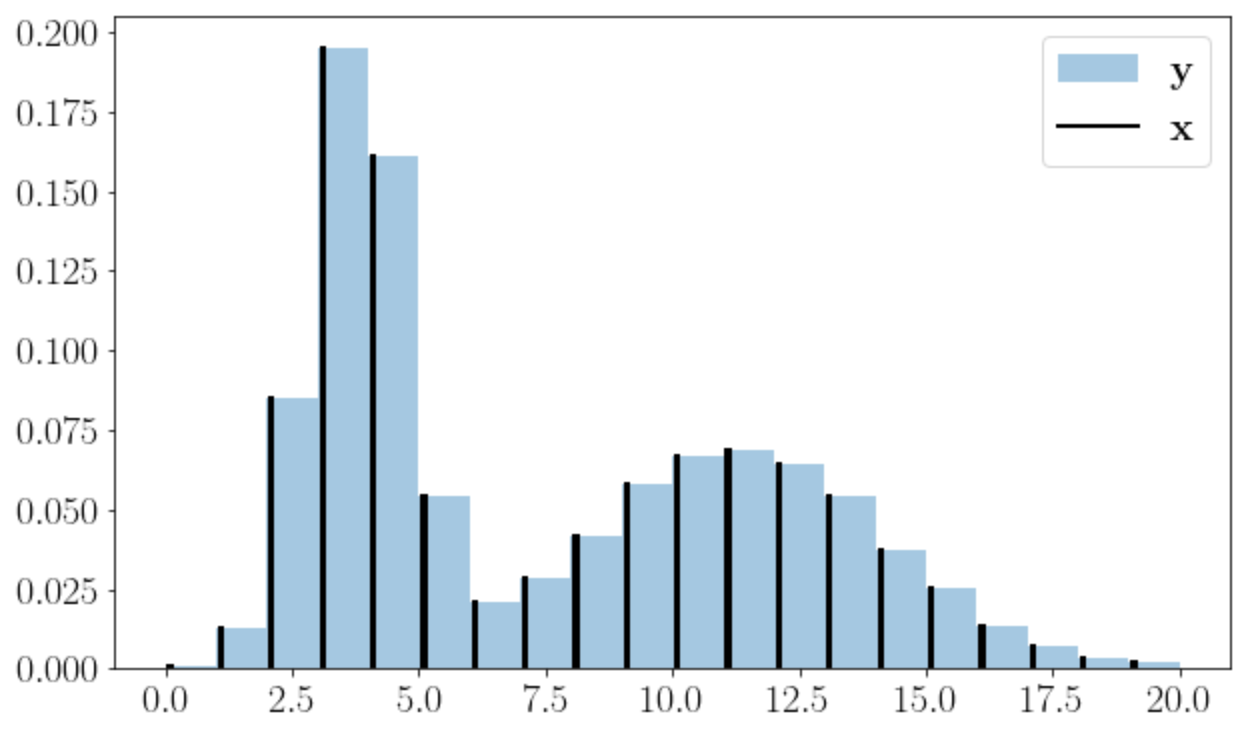
\includegraphics[width=1.0\linewidth]{figs/uniform_dequantization.png}
			\end{figure}
	\end{minipage}%
	\begin{minipage}[t]{0.5\columnwidth}
		\begin{figure}
			\centering
			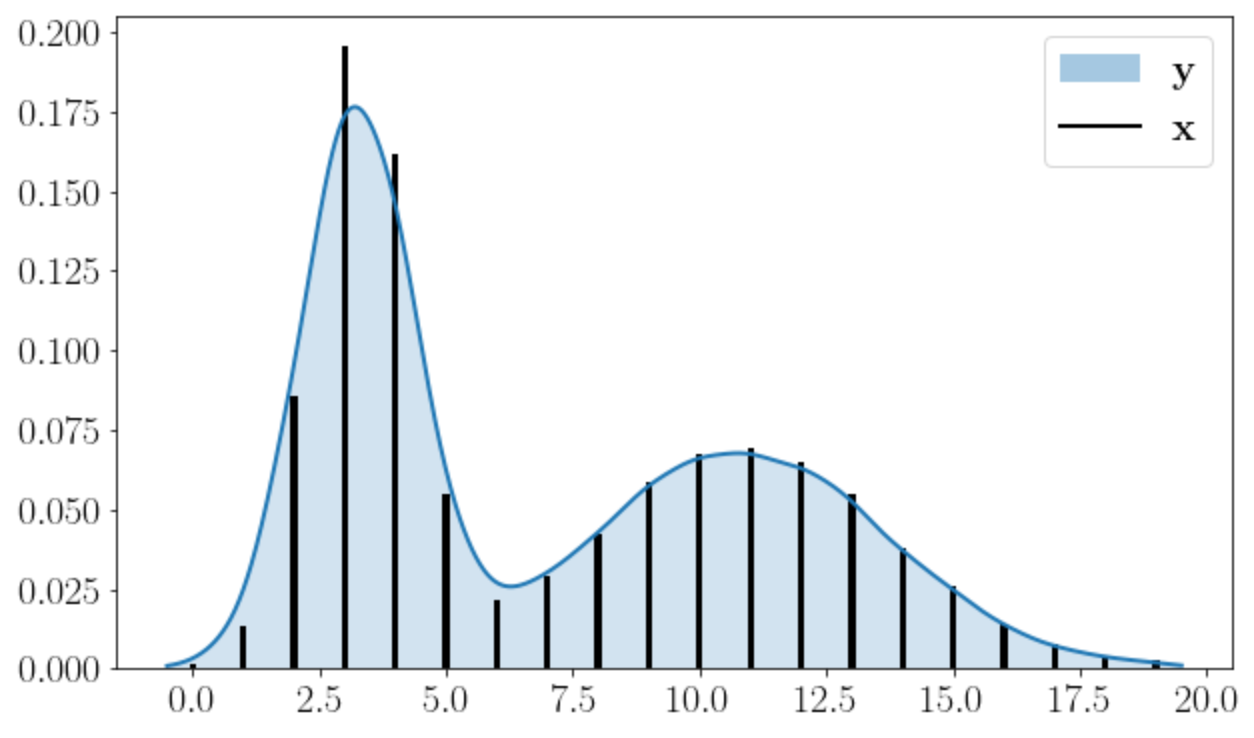
\includegraphics[width=1.0\linewidth]{figs/variational_dequantization.png}
		\end{figure}
	\end{minipage}
	\begin{itemize}
		\item $p(\by | \btheta)$ assign unifrom density to unit hypercubes $\bx + U[0, 1]$ (left fig).
		\item Neural network density models is a smooth function approximator (right fig).
		\item Smooth dequantization is more natural.
	\end{itemize}
	How to make the smooth dequantization? \\
\end{frame}
%=======
\begin{frame}{Flow++}
	\begin{block}{Variational dequantization}
		Introduce variational dequantization noise distribution $q(\bu | \bx)$ and treat it as an approximate posterior. 
	\end{block}
	\begin{block}{Variational lower bound}
		\begin{multline*}
			\log P(\bX | \btheta) = \sum_{i=1}^n \log P(\bx_i | \btheta) = \sum_{i=1}^n \left[ \log \int q(\bu | \bx) \frac{p(\bx + \bu | \btheta)}{q(\bu | \bx)} d \bu \right] \geq \\ 
			\geq\sum_{i=1}^n \left[  \int q(\bu | \bx) \log \frac{p(\bx + \bu | \btheta)}{q(\bu | \bx)} d \bu \right] = \\ = \int q(\bU | \bX) \log \frac{p(\bX + \bU | \btheta)}{q(\bU | \bX)} d \bU = \mathcal{L}(q, \btheta).
		\end{multline*}
	\end{block}
	\myfootnotewithlink{https://arxiv.org/abs/1902.00275}{Ho J. et al. Flow++: Improving Flow-Based Generative Models with Variational Dequantization and Architecture Design, 2019}
\end{frame}
%=======
\begin{frame}{Flow++}
	\begin{block}{Variational lower bound}
		\[
		\mathcal{L}(q, \btheta) = \int q(\bU | \bX) \log \frac{p(\bX + \bU | \btheta)}{q(\bU | \bX)} d \bU.
		\]
	\end{block}
	Let $\bu = h(\bepsilon)$ is a flow model with base distribution $\bepsilon \sim p(\bepsilon) = \mathcal{N}(0, \mathbf{I})$:
	\[
		q(\bu | \bx) = p(h^{-1}(\bu)) \cdot \left| \det \frac{\partial h^{-1}(\bu)}{\partial \bu}\right|.
	\]
	Then
	\[
		\log P(\bX | \btheta) \geq \sum_{i=1}^n \int \log \left( \frac{p(\bx + h(\bepsilon))}{p(\bepsilon) \cdot \left| \det \frac{\partial h(\bepsilon)}{\partial \bepsilon}\right|^{-1}} \right) d\bepsilon.
	\]
	\myfootnotewithlink{https://arxiv.org/abs/1902.00275}{Ho J. et al. Flow++: Improving Flow-Based Generative Models with Variational Dequantization and Architecture Design, 2019}
\end{frame}
%=======
\begin{frame}{Flow++}
	\[
		\log P(\bX | \btheta) \geq \sum_{i=1}^n \int \log \left( \frac{p(\bx + h(\bepsilon))}{p(\bepsilon) \cdot \left| \det \frac{\partial h(\bepsilon)}{\partial \bepsilon}\right|^{-1}} \right) d\bepsilon.
	\]
	If $p(\bx + \bu | \btheta)$ is also a flow model, it is straightforward to calculate stochastic gradient of this ELBO.
	
	\textbf{Note:} Uniform dequantization is a special case of variational dequantization ($q(\bu | \bx) = U[0, 1]$).
	The gap between $\log P(\bX | \btheta)$ and the derived ELBO is 
	\[
		KL(q(\bU | \bX) || p(\bU | \bX)).
	\]
	In the case of uniform dequantization the model unnaturally places uniform density over each hypercube $\bx + U[0, 1]$ due to inexpressive distribution $q$.
	\myfootnotewithlink{https://arxiv.org/abs/1902.00275}{Ho J. et al. Flow++: Improving Flow-Based Generative Models with Variational Dequantization and Architecture Design, 2019}
\end{frame}
%=======
\begin{frame}{Flow++}
	\begin{figure}
		\centering
		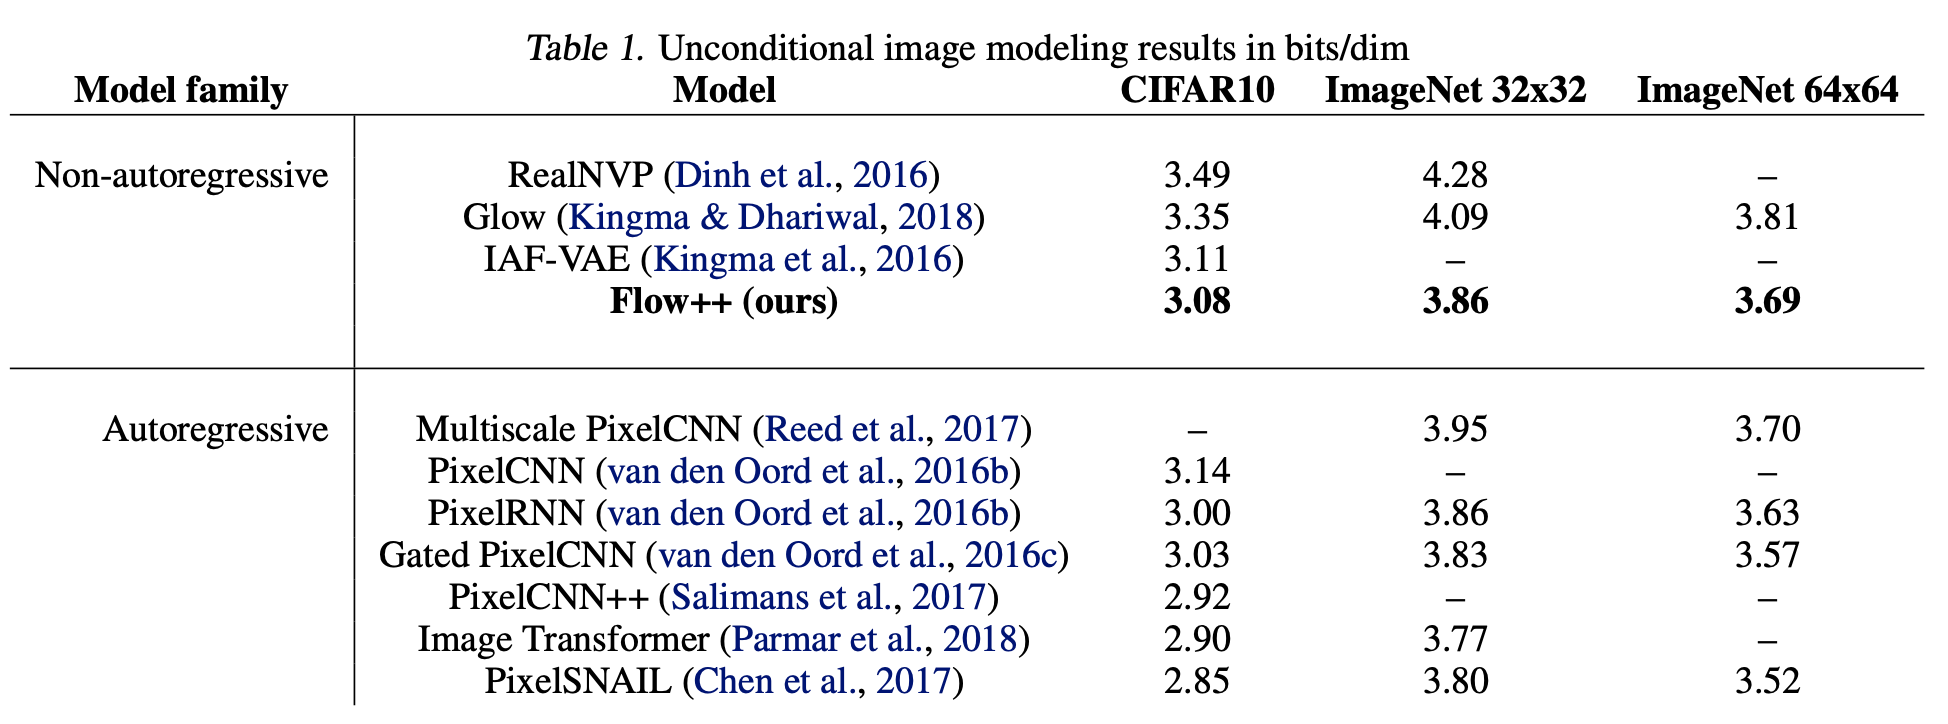
\includegraphics[width=0.7\linewidth]{figs/flow++1.png}
	\end{figure}
	\vspace{-0.1cm}
	\begin{figure}
		\centering
		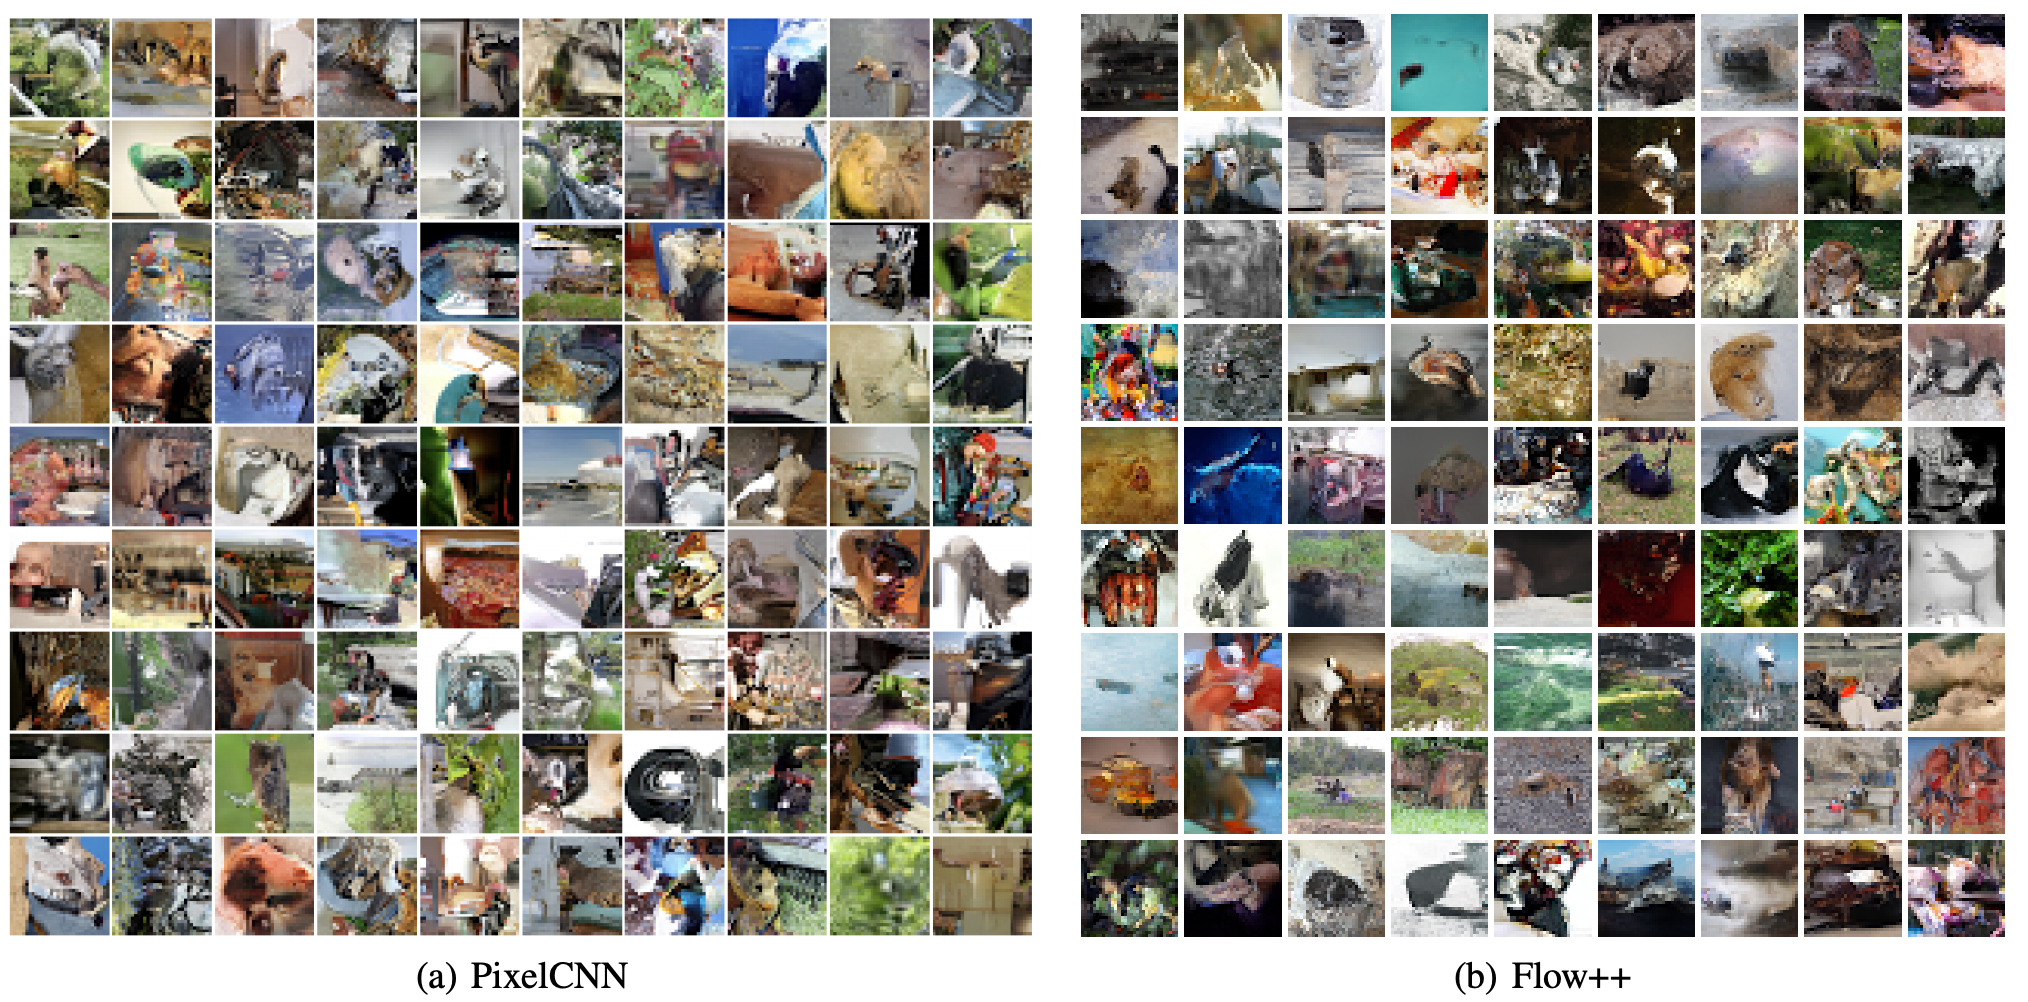
\includegraphics[width=0.8\linewidth]{figs/flow++2.png}
	\end{figure}
	\myfootnotewithlink{https://arxiv.org/abs/1902.00275}{Ho J. et al. Flow++: Improving Flow-Based Generative Models with Variational Dequantization and Architecture Design, 2019}
\end{frame}
%=======
%--------------------------------------------------------------------------------
\begin{frame}{Likelihood-based models}
	\begin{block}{Exact likelihood evaluation}
		\begin{itemize}
			\item Autoregressive models (PixelCNN, WaveNet);
			\item Flow models (NICE, RealNVP, Glow).
		\end{itemize}
	\end{block}
	\begin{block}{Approximate likelihood evaluation}
		\begin{itemize}
			\item Latent variable models (VAE).
		\end{itemize}
	\end{block}
	What are the pros and cons of each of them? \\
	\vspace{0.2cm}
\end{frame}
%=======
\begin{frame}{VAE recap}
	\vspace{-0.5cm}
	\[
	p(\bx | \btheta) \geq \mathcal{L} (\bphi, \btheta)  = \mathbb{E}_{q(\bz | \bx, \bphi)} \log \frac{p(\bx, \bz | \btheta)}{q(\bz| \bx, \bphi)} \rightarrow \max_{\bphi, \btheta}.
	\]
	\vspace{-0.5cm}
	\begin{figure}[h]
		\centering
		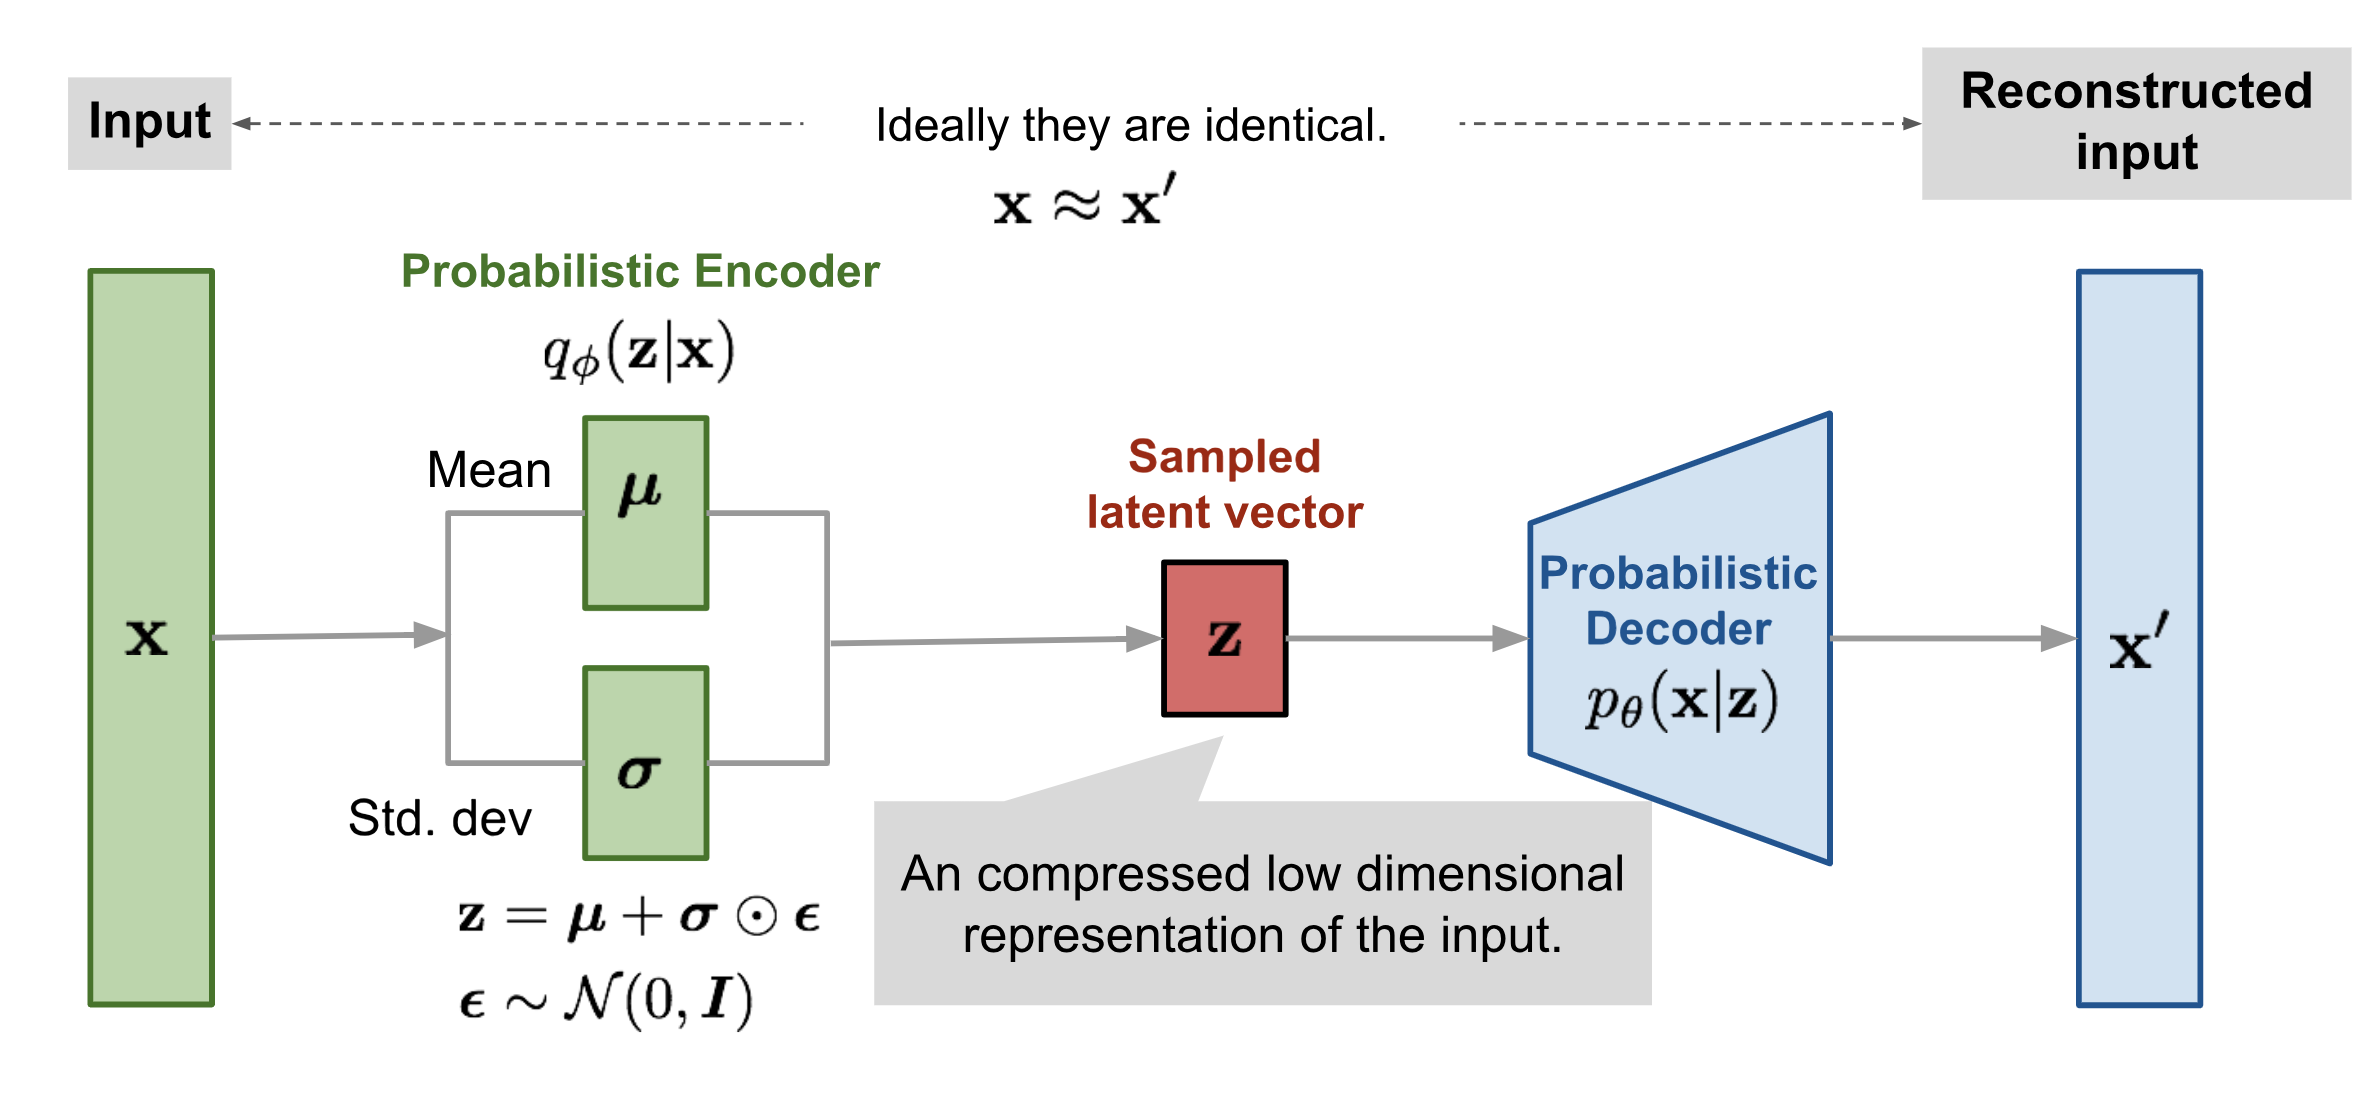
\includegraphics[width=\linewidth]{figs/vae-gaussian.png}
	\end{figure}
	\myfootnotewithlink{https://lilianweng.github.io/lil-log/2018/08/12/from-autoencoder-to-beta-vae.html}{image credit: https://lilianweng.github.io/lil-log/2018/08/12/from-autoencoder-to-beta-vae.html}
	
\end{frame}
%=======
\begin{frame}{VAE limitations}
	\begin{itemize}
		\item Poor variational posterior distribution (encoder)
		\[
		q(\bz | \bx, \bphi) = \mathcal{N}(\bz| \bmu_{\bphi}(\bx), \bsigma^2_{\bphi}(\bx)).
		\]
		\item Poor prior distribution
		\[
		p(\bz) = \mathcal{N}(0, \mathbf{I}).
		\]
		\item Poor probabilistic model (decoder)
		\[
		p(\bx | \bz, \btheta) = \mathcal{N}(\bx| \bmu_{\btheta}(\bz), \bsigma^2_{\btheta}(\bz)).
		\]
		\item Loose lower bound
		\[
		p(\bx | \btheta) - \mathcal{L}(q, \btheta) = (?).
		\]
	\end{itemize}
\end{frame}
%=======
\begin{frame}{Variational posterior}
	
	We wish $KL(q(\bz | \bx, \bphi) || p(\bz | \bx, \btheta)) = 0$. \\
	(In this case the lower bound is tight $p(\bx | \btheta) = \mathcal{L}(q, \btheta)$). \\
	\vspace{0.5cm}
	Normal variational distribution $q(\bz | \bx, \bphi) = \mathcal{N}(\bz| \bmu_{\bphi}(\bx), \bsigma^2_{\bphi}(\bx))$ is poor (e.g. has only one mode). \\
	\vspace{0.5cm}
	Flows models convert a simple base distribution to a compex one using invertible transformation with simple Jacobian. \\
	\vspace{0.5cm}
	How to use flows in VAE?
\end{frame}
%=======
\begin{frame}{Flows in VAE}
	Apply a sequence of transformations to the random variables 
	\[
	\bz_0 \sim q(\bz | \bx, \bphi) = \mathcal{N}(\bz| \bmu_{\bphi}(\bx), \bsigma^2_{\bphi}(\bx)).
	\]
	Here, $q(\bz | \bx, \bphi)$ (which is a VAE encoder) plays a role of a base distribution.
	\[
	\bz_0 \xrightarrow{g_1} \bz_1 \xrightarrow{g_2} \dots \xrightarrow{g_K} \bz_K, \quad \bz_K = g(\bz_0), \quad g = g_K \circ \dots \circ g_1.
	\]
	Each $g_k $ is a flow transformation (e.g. planar, radial, coupling layer) parameterized by $\bphi_k$.
	\begin{align*}
		\log q_K(\bz_K | \bx, \bphi, \{\bphi\}_{k=1}^K) &= \log q(\bz_0 | \bx, \bphi) \\ &- \sum_{k=1}^K \log \left| \det \left( \frac{\partial g_k(\bz_{k - 1}, \bphi_k)}{\partial \bz_{k-1}} \right) \right|.
	\end{align*}
	
	\vfill
	\hrule\medskip
	{\scriptsize \href{https://arxiv.org/pdf/1505.05770.pdf}{https://arxiv.org/pdf/1505.05770.pdf}} 
\end{frame}
%=======
\begin{frame}{Flows in VAE}
	\begin{block}{Flow model in latent space}
		\vspace{-0.5cm}
		\begin{align*}
			\log q_K(\bz_K | \bx, \bphi, \{\bphi\}_{k=1}^K) &= \log q(\bz_0 | \bx, \bphi) \\ &- \sum_{k=1}^K \log \left| \det \left( \frac{\partial g_k(\bz_{k - 1}, \bphi_k)}{\partial \bz_{k-1}} \right) \right|.
		\end{align*}
		\vspace{-0.5cm}
	\end{block}
	Let use $q_K(\bz_K | \bx, \bphi_*), \, \bphi_* = \{\bphi, \bphi_1, \dots, \bphi_K\}$ as a variational distribution. \\
	Here $\bphi$~-- encoder parameters, $\{\bphi\}_{k=1}^K$~-- flow parameters.
	\begin{block}{ELBO objective}
		\vspace{-0.5cm}
		\begin{align*}
			\mathcal{L} (\bphi, \btheta)  &= \mathbb{E}_{q_K(\bz_K | \bx, \bphi_*)} \log \frac{p(\bx, \bz_K | \btheta)}{q_K(\bz_K| \bx, \bphi_*)} \\
			&= \mathbb{E}_{q_K(\bz_K | \bx, \bphi_*)} \bigl[\log p(\bx, \bz_K | \btheta) - \log q_K(\bz_K| \bx, \bphi_*) \bigr] 
		\end{align*}
	\end{block}
	\vfill
	\hrule\medskip
	{\scriptsize \href{https://arxiv.org/pdf/1505.05770.pdf}{https://arxiv.org/pdf/1505.05770.pdf}} 
\end{frame}
%=======
\begin{frame}{Flows in VAE}
	\begin{block}{Variational distribution}
		\vspace{-0.5cm}
		\[
			\log q_K(\bz_K | \bx, \bphi_*) = \log q(\bz_0 | \bx, \bphi) - \sum_{k=1}^K \log \left| \det \left( \frac{\partial g_k(\bz_{k - 1}, \bphi_k)}{\partial \bz_{k-1}} \right) \right|.
		\]
		\vspace{-0.5cm}
	\end{block}
	\begin{block}{ELBO objective}
		\vspace{-0.5cm}
		\begin{align*}
			\mathcal{L} (\bphi, \btheta) 
			&= \mathbb{E}_{q_K(\bz_K | \bx, \bphi_*)} \bigl[\log p(\bx, \bz_K | \btheta) - \log q_K(\bz_K| \bx, \bphi_*) \bigr] \\
			&= \mathbb{E}_{q(\bz_0 | \bx, \bphi)} \left. \bigl[\log p(\bx, \bz_K | \btheta) - \log q_K(\bz_K| \bx, \bphi_*) \bigr]\right|_{\bz_K = g(\bz_0, \{\bphi\}_{k=1}^K)} \\
			&= \mathbb{E}_{q(\bz_0 | \bx, \bphi)} \bigg[\log p(\bx, \bz_K | \btheta) -  \log q(\bz_0 | \bx, \bphi ) + \\ & + \sum_{k=1}^K \log \left| \det \left( \frac{\partial g_k(\bz_{k - 1}, \bphi_k)}{\partial \bz_{k-1}} \right) \right| \bigg].
		\end{align*}
	\end{block}
	\myfootnotewithlink{https://arxiv.org/abs/1505.05770}{Rezende D. J., Mohamed S. Variational Inference with Normalizing Flows, 2015} 
\end{frame}
%=======
\begin{frame}{Gaussian autoregressive model}
	Consider autoregressive model
	\[
		p(\bx | \btheta) = \prod_{i=1}^m p(x_i | \bx_{1:i - 1}, \btheta),
	\]
	with conditionals
	\[
	p(x_i | \bx_{1:i - 1}, \btheta) = \mathcal{N} \left(\hat{\mu}_i(\bx_{1:i-1}), \hat{\sigma}^2_i (\bx_{1:i-1})\right).
	\]
	\vspace{-0.5cm}
	\begin{block}{Sampling}
		\[
		x_i = \hat{\sigma}_i (\bx_{1:i-1}) \cdot z_i + \hat{\mu}_i(\bx_{1:i-1}), \quad z_i \sim \mathcal{N}(0, 1).
		\]
	\end{block}
	Sampling from autoregressive model is sequential. \\
	Note that we could interpret this sampling as a transformation $\bx = g(\bz, \btheta)$, where $\bz$ comes from base distribution $\mathcal{N}(0, 1)$.
\end{frame}
%=======
\begin{frame}{Gaussian autoregressive model}
	\begin{block}{Sampling}
		\vspace{-0.5cm}
		\[
		x_i = \hat{\sigma}_i (\bx_{1:i-1}) \cdot z_i + \hat{\mu}_i(\bx_{1:i-1}), \quad z_i \sim \mathcal{N}(0, 1).
		\]
		\vspace{-0.5cm}
	\end{block}
	\begin{block}{Jacobian}
		\vspace{-0.5cm}
		\[
		\log \left|\det \left( \frac{\partial f(\bx, \btheta)}{\partial \bx} \right) \right| = -\log \left|\det \left( \frac{\partial g(\bz, \btheta)}{\partial \bz} \right) \right| = - \sum_{i = 1}^m \log \hat{\sigma}_i (\bx_{1:i-1}).
		\]
		\vspace{-0.5cm}
	\end{block} 
	\begin{block}{Inverse transform}
		\vspace{-0.5cm}
		\[
		z_i = \left(x_i - \hat{\mu}_i(\bx_{1:i-1}) \right) \cdot \frac{1}{\hat{\sigma}_i (\bx_{1:i-1}) }.
		\]
	\end{block}
	We get an autoregressive model with tractable (triangular) Jacobian, which is easily invertible. It is a flow!
\end{frame}
%=======
\begin{frame}{Inverse autoregressive flow (IAF)}
	
	\begin{block}{Gaussian autoregressive model ($\bz \rightarrow \bx$)}
		\vspace{-0.2cm}
		\[
			x_i = \hat{\sigma}_i (\bx_{1:i-1}) \cdot z_i + \hat{\mu}_i(\bx_{1:i-1}).
		\]
		\[
			z_i = \left(x_i - \hat{\mu}_i(\bx_{1:i-1}) \right) \cdot \frac{1}{ \hat{\sigma}_i (\bx_{1:i-1})}.
		\]
		\vspace{-0.3cm}
	\end{block}
	This process is sequential. \\
	Let use the following reparametrization:
	$\bsigma = \frac{1}{\hat{\bsigma}}; \quad \bmu = - \frac{\hat{\bmu}}{\hat{\bsigma}}.$
	
	\begin{block}{Inverse transform ($\bx \rightarrow \bz$)}
		\vspace{-0.2cm}
		\[
			z_i = \sigma_i (\bx_{1:i-1}) \cdot x_i + \mu_i(\bx_{1:i-1}).
		\]
		\[
			x_i = \left( z_i - \mu_i(\bx_{1:i-1})\right) \cdot \frac{1}{\sigma_i (\bx_{1:i-1}) }.
		\]
		\vspace{-0.3cm}
	\end{block}
	This process is \textbf{not} sequential.
	\myfootnotewithlink{https://arxiv.org/abs/1606.04934}{Kingma D. P. et al. Improving Variational Inference with Inverse Autoregressive Flow, 2016} 
\end{frame}
%=======
\begin{frame}{Inverse autoregressive flow (IAF)}
	
	\begin{block}{Inverse transform ($\bx \rightarrow \bz$)}
		\vspace{-0.2cm}
		\[
			z_i = \sigma_i (\bx_{1:i-1}) \cdot x_i + \mu_i(\bx_{1:i-1}).
		\]
		\[
			x_i = \left( z_i - \mu_i(\bx_{1:i-1})\right) \cdot \frac{1}{\sigma_i (\bx_{1:i-1})}.
		\]
		\vspace{-0.3cm}
	\end{block}
	Inverse autoregressive flow use such inverted autoregressive model as a flow in VAE:
	\begin{align*}
		\bz_0 &= \bsigma(\bx) \cdot \bepsilon + \bmu(\bx), \quad \bepsilon \sim \mathcal{N}(0, 1); \quad  \sim q(\bz_0 | \bx, \bphi). \\
		\bz_k &= \bsigma_k(\bz_{k - 1}) \cdot \bz_{k-1} + \bmu_k(\bz_{k - 1}), \quad k \geq 1; \quad  \sim q_k(\bz_k | \bx, \bphi, \{\bphi_j\}_{j=1}^k).
	\end{align*}
	\myfootnotewithlink{https://arxiv.org/abs/1606.04934}{Kingma D. P. et al. Improving Variational Inference with Inverse Autoregressive Flow, 2016} 
\end{frame}
%=======
\begin{frame}{Flows}
	\begin{figure}
		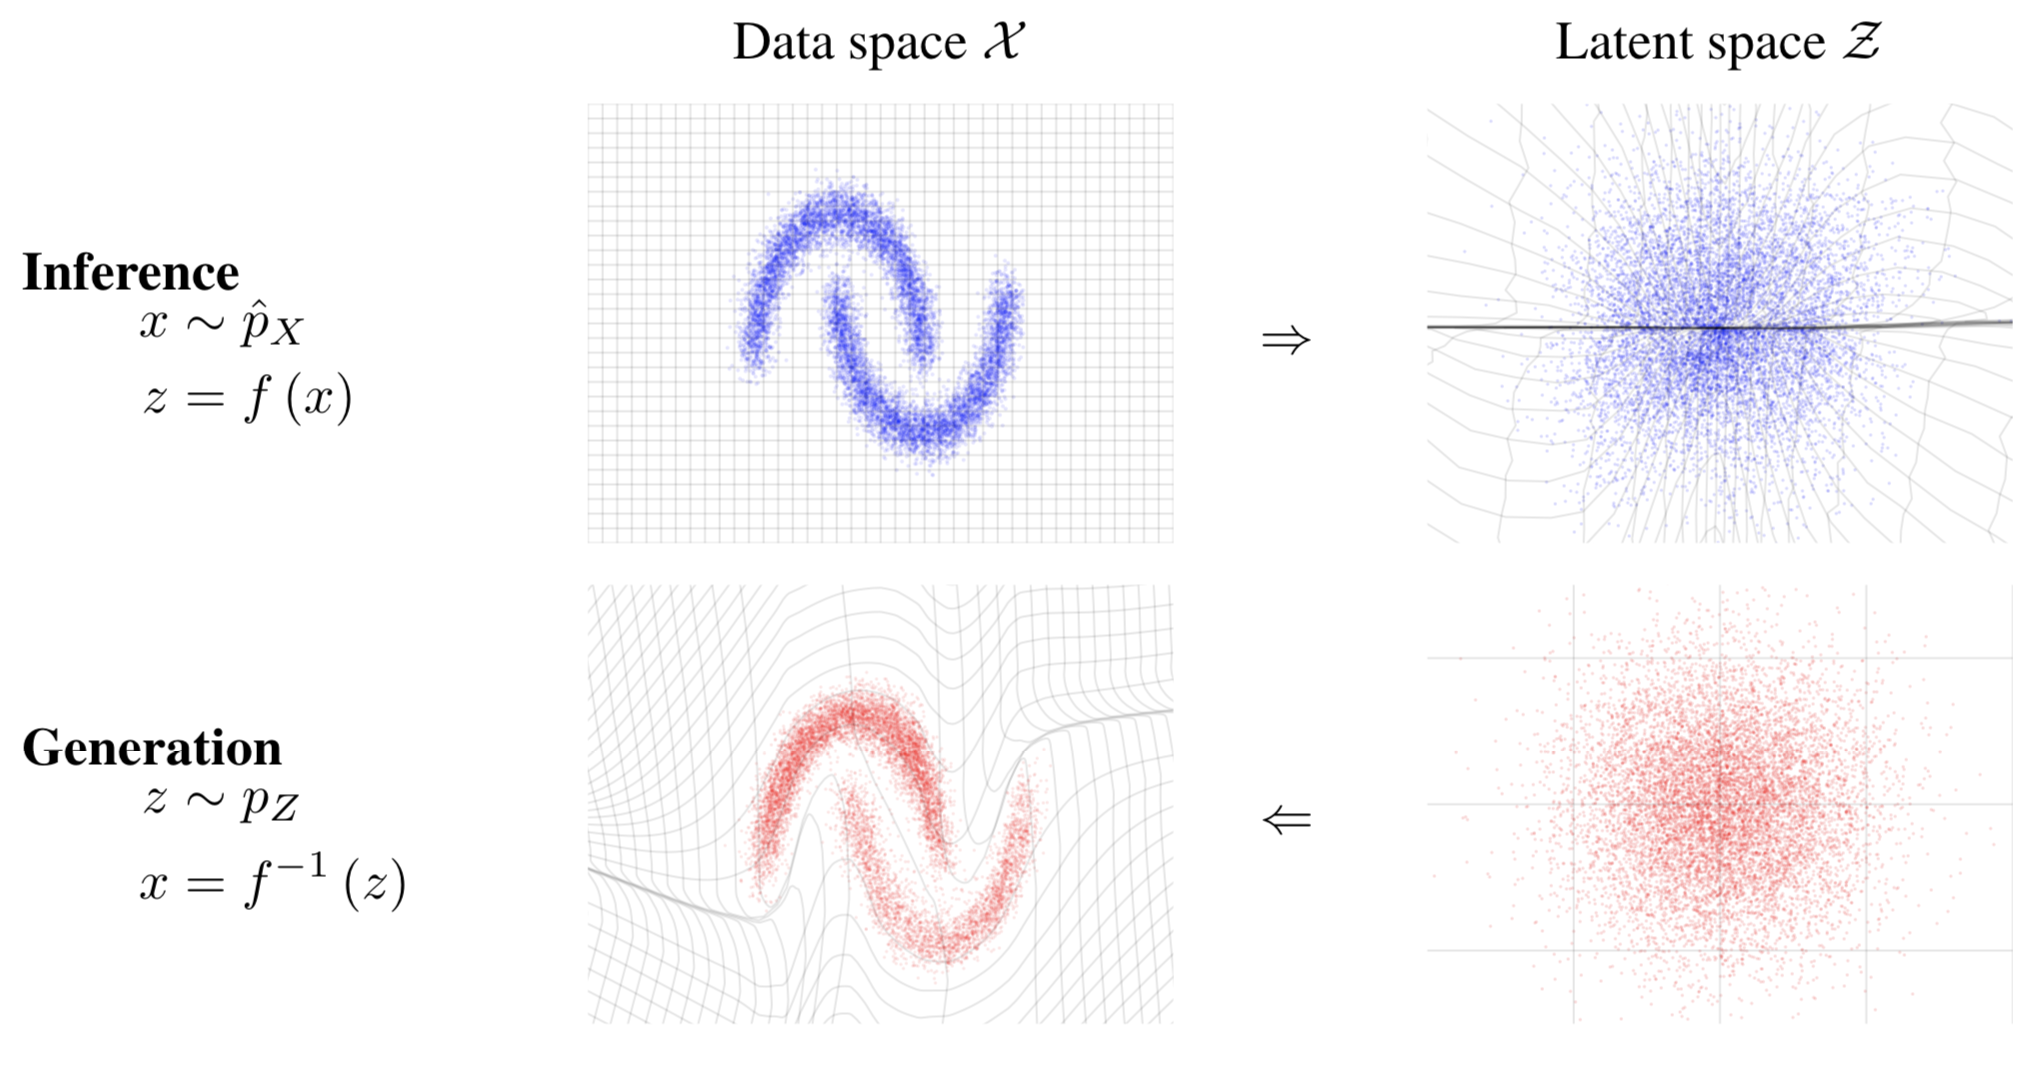
\includegraphics[width=0.8\linewidth]{figs/flows_how2.png}
	\end{figure}
	\begin{itemize}	
		\item Inference mode in autoregressive flows is used for density estimation tasks.
		\item Generation mode in autoregressive flows (IAF) is used for stochastic variational inference to get a more flexible posterior distribution.
	\end{itemize}

	\myfootnotewithlink{https://arxiv.org/abs/1605.08803}{Dinh L., Sohl-Dickstein J., Bengio S. Density estimation using Real NVP, 2016} 
\end{frame}
%=======
\begin{frame}{Inverse autoregressive flow (IAF)}
	\begin{figure}
		\includegraphics[width=\linewidth]{figs/iaf2.png}
	\end{figure}
	\begin{figure}
		\includegraphics[width=\linewidth]{figs/iaf1.png}
	\end{figure}

	\myfootnotewithlink{https://arxiv.org/abs/1606.04934}{Kingma D. P. et al. Improving Variational Inference with Inverse Autoregressive Flow, 2016} 
\end{frame}
%=======
\begin{frame}{Summary}
\begin{itemize}
	\item Planar flows is a simple form of an invertible flow model (Sylvester flows are their extension). The NICE model is a more powerful type of flow.
\end{itemize}
\end{frame}
\end{document} 